\documentclass[a4paper,12pt]{report}

\usepackage[margin=1in]{geometry}
\usepackage{alltt, fancyvrb, url}
\usepackage{graphicx}
\usepackage{subfigure}
\usepackage{wrapfig}
\usepackage{algorithmic}
\usepackage[utf8]{inputenc}
\usepackage{fontenc}
\usepackage{amsmath,stmaryrd,mathtools,algorithm}
\usepackage{amssymb}
\usepackage{float}
\usepackage{hyperref}
\usepackage[italian]{cleveref}
\usepackage[italian]{babel}


\title{Relazione progetto OOPang}
\author{Samuele Burattini \\ Nicholas Ciarafoni \\ Francesco Dente \\ Lorenzo Menghini \\ Francesca Tonetti}
\date{\today}

\begin{document}
 
\maketitle

\tableofcontents

\chapter{Analisi}

Lo scopo del progetto è di realizzare un clone del gioco arcade Pang, nel quale uno o due giocatori hanno l'obiettivo di distruggere le palle generate dal gioco senza essere colpiti.
Queste palle si sdoppiano dimezzando la loro dimensione ogni volta che vengono colpite da un proiettile, fino a scomparire ad una dimensione minima prefissata.
Ad ogni collisione con il pavimento le palle rimbalzano tornando sempre alla stessa altezza a seconda della loro dimensione (le più grandi in alto, quelle più piccole più in basso).

\section{Requisiti}

\subsubsection{Requisiti funzionali}
\begin{itemize}
	\item L'applicazione dovrà emulare fedelmente il gioco rispettando collisioni e gravità annessa in modo "naturale".
	\item L'utente potrà scegliere due modalità di gioco: una "Tour Mode" composta da 17 livelli a tempo con difficoltà crescente, o la modalità "Survival" dove l'utente ha come obiettivo di resistere il più a lungo possibile.
	\item L'utentè potrà scegliere se giocare da solo o in modalità multiplayer collaborativo con l'utilizzo della tastiera condivisa.
	\item Durante un livello, il giocatore potrà raccogliere dei potenziamenti che modificano lo stato del gioco (scudo protettivo, doppio sparo, ecc...).
	\item L'applicazione potrà gestire più profili utente mediante un login con password in modo da conservare i dati in maniera permantente tra una sessione di gioco e l'altra.
	\item L'utente accumulerà ad ogni partita un punteggio che verrà convertito in punti esperienza, utili ad avanzare il proprio rank e guadagnare monete.
	\item L'utente potrà spendere i coins guadagnati durante le partite per incrementare il livello dei potenziamenti rendendoli più efficaci.
	\item L'applicazione terrà traccia dei punteggi di tutti gli utenti registrati sulla stessa macchina mostrando i migliori 10 al termine di ogni sessione di gioco.
\end{itemize}

\subsubsection{Requisiti non funzionali}
\begin{itemize}
	\item L'applicazione dovrà essere efficiente nella gestione e caricamento delle risorse grafiche.
	\item L'applicazione dovrà gestire la memoria persistente tramite salvataggio su file.
	\item L'applicazione dovrà garantire ua sicurezza minima sulle password di ogni utente.
	\item L'applicazione dovrà poter caricare i livelli precedentemente scritti e studiati ad hoc dagli sviluppatori.
\end{itemize}

\section{Analisi e modello del dominio}

L'entità base del modello del dominio è il Level, in cui agiscono tutti i componenti del gioco rappresentati dai GameObject.
Quest'ultimi descrivono gli "attori" fondamentali che compongono il gioco quali balls, player/s, walls, shots e pickups e sono completamente responsabili del proprio comportamento.
Il Level ha la responsabilità di mantenere attivi e aggiornati i componenti al suo interno mediante update incrementali che comunicano il trascorrere del tempo.
All'interno del level è presente un motore per la gestione delle collisioni tra gli oggetti in gioco: ogni GameObject oltre alla logica del proprio comportamento può includere un Collidable che gli permette di essere rilevato dal CollisionManager e di essere notificato quando colpisce altri oggetti.
Essendo il level un'entità che varia duarante il gioco, esso viene incapsulato all'interno del Model che permette di modificarlo durante la sessione di gioco.
La complessità nella realizzazione del dominio sarà gestire in maniera efficacie le collisioni tra gli oggetti e l'aggiornamento coerente di tutti i GameObject.

\begin{figure}[H]
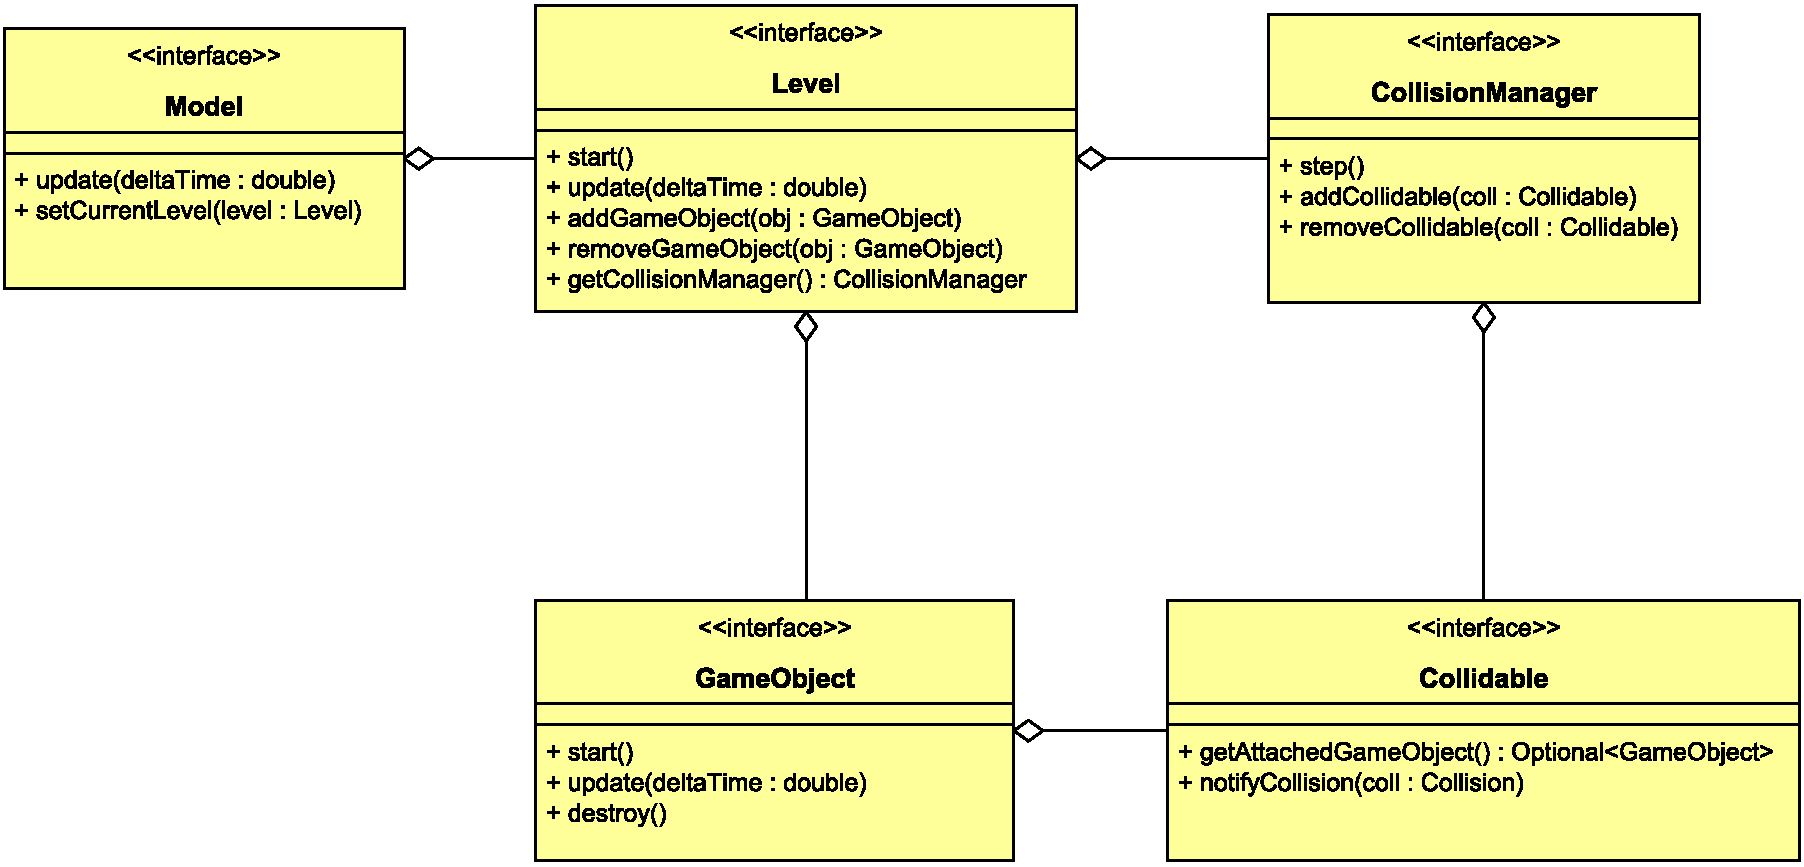
\includegraphics[width=\linewidth]{img/model}
\caption{Schema UML del modello del dominio.}
\label{img:model}
\end{figure}

\chapter{Design}

\section{Architettura}

Abbiamo scelto di utilizzare il pattern architetturale MVC per l'applicazione, in quanto uno dei pattern visti a lezione e perchè ci ha permesso di separare in maniera efficacie la logica di gioco dalle feature grafiche.
Nel nostro caso abbiamo creato un'interfaccia per ogni ambito in modo da semplificare le relazioni tra di esse.

\begin{figure}[H]
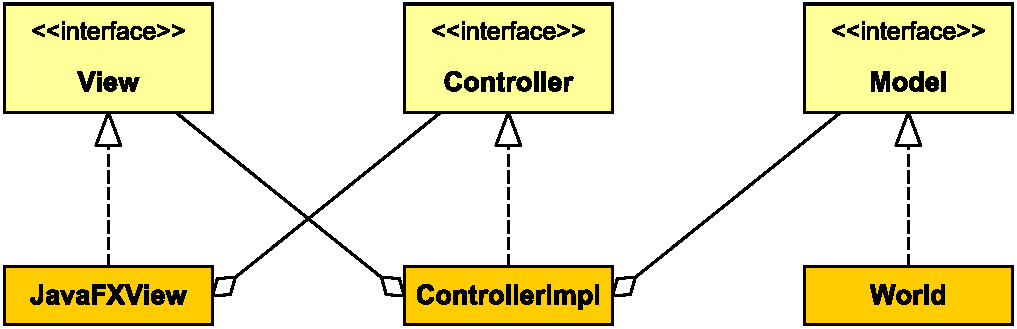
\includegraphics[width=\linewidth]{img/mvc}
\caption{Schema UML dell'architettura generale dell'applicazione e del pattern MVC.}
\label{img:mvc}
\end{figure}

In particolare l'interfaccia Model nasconde la logica in-game e la descrizione delle varie entità e di come interagiscono all'interno del Level.
Nella progettazione di questa componente abbiamo fatto in modo che fosse chiusa in se stessa.
Abbiamo dunque cercato di tenerla all'oscuro dell'esistenza di view e controller, rendendo quest'ultime responsabili di chiedere le informazioni necessarie.
Come mostrato nella \Cref{img:mvc} infatti, la componente Model non ha alcun riferimento alle altre componenti.

Nel Controller abbiamo inserito la gestione del flusso di utilizzo del software e dell'accesso ai dati persistenti (users e leaderboard).
Il suo compito principale è mantenere un'astrazione di GameSession (serie di livelli che termina all'esaurimento delle vite).
Ogni sessione apre per ogni livello un gestore del loop che aggiorna periodicamente il model, rappresentato dall'interfaccia GameLoop.

\begin{figure}[H]
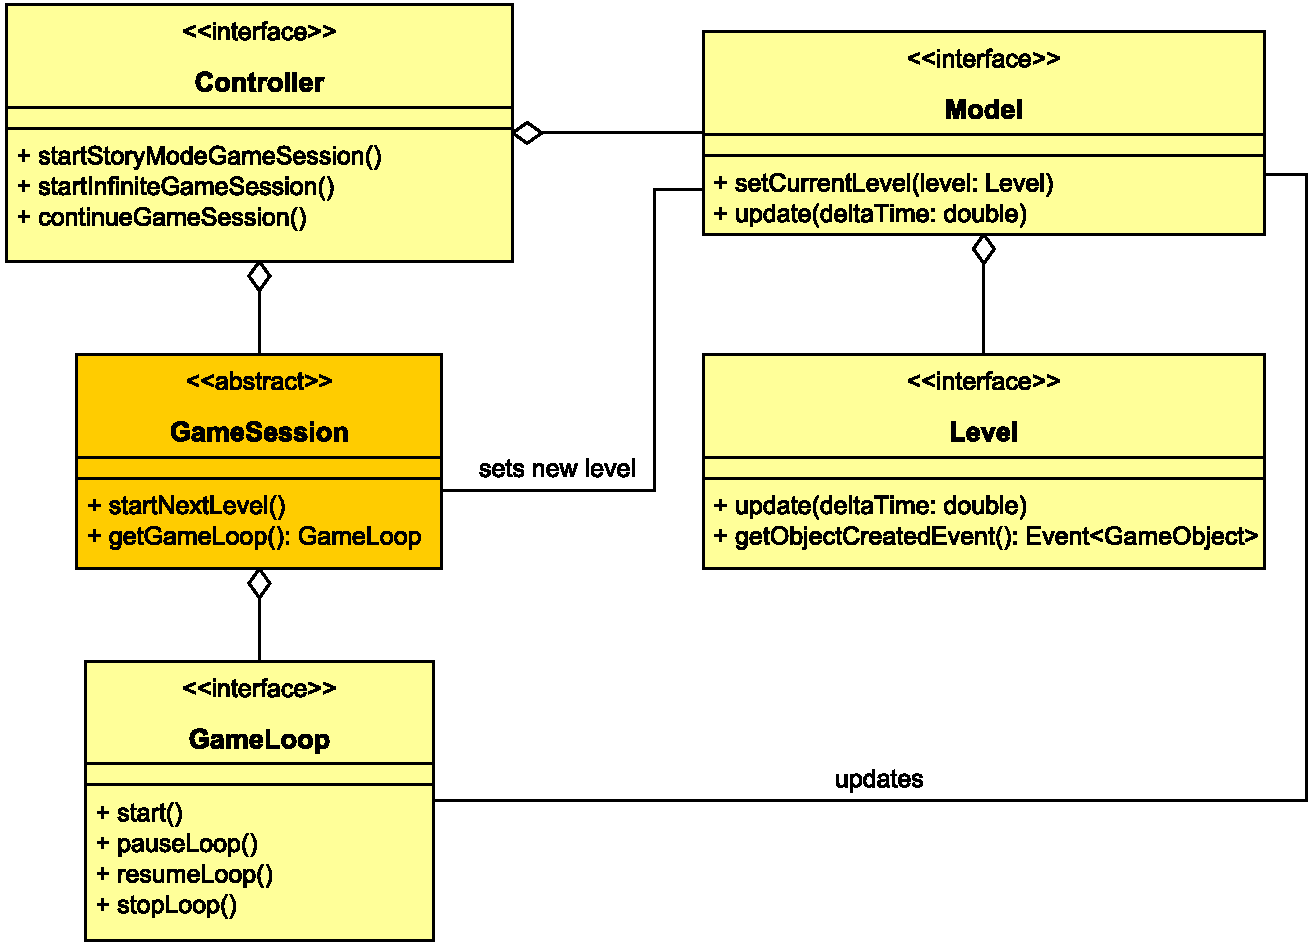
\includegraphics[width=\linewidth]{img/model_controller}
\caption{Schema UML che mostra l'interazione tra Controller e Model.}
\label{img:model_controller}
\end{figure}

Per quanto riguarda l'interazione con l'utente, la View si occupa della visualizzazione delle schermate dell'applicativo e nella fase di gioco del rendering del mondo.
Il metodo loadScene() modifica la schermata correntemente visualizzata, permettendo al controller di richiedere un cambio di scena.
Il rendering del mondo viene affidato al CanvasDrawer, componente della View il cui compito è la visualizzazione grafica effettiva del modello.
La richiesta di renderizzazione è effettuata dal GameLoop in seguito ad ogni fase di update del Model in modo da rispecchiare i cambiamenti avvenuti.

CanvasDrawer e Level svolgono dunque ruoli paralleli nei rispettivi ambiti dell'MVC, mantenendo aggiornati gli oggetti attivi e propagando le richieste del GameLoop su ognuno di essi.
Per questo motivo il CanvasDrawer svolge il ruolo di Observer nei confronti del Level, ottenendo così uno stato coerente tra parte logica e parte grafica.

\begin{figure}[H]
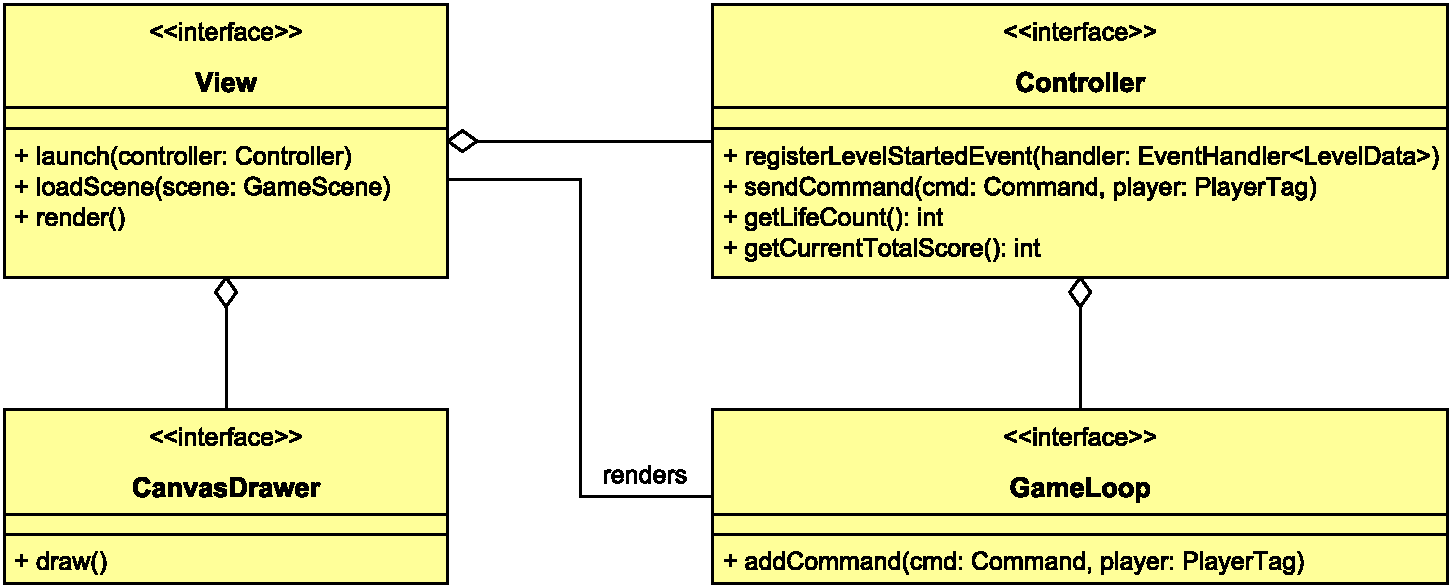
\includegraphics[width=\linewidth]{img/controller_view}
\caption{Schema UML che mostra l'interazione tra Controller e View.}
\label{img:controller_view}
\end{figure}

\section{Design dettagliato}

\subsection*{Samuele Burattini}

\subsubsection*{Shooting}

Per modellare l'azione di sparo di un proiettile ho identificato tre responsabiltà principali e ho deciso di affidarle a oggetti distinti per avere la massima flessibilità.

La responsabilità di creazione del proiettile è stata affidata all'interfaccia Shooter che descrive oggetti dotati di posizione e di un Supplier di Shot che gli permette di istanziare nuovi oggetti a partire appunto dalla posizione corrente dello Shooter stesso.

Allo ShooterComponent è affidato invece il compito di inviare le richieste fatte dal GameObject di cui fa parte lo Shooter e anche di mantenere quest'ultimo aggiornato alla posizione del GameObject.
Lo ShooterComponent utilizza lo Shooter via Strategy e può settare il suo stato a seconda se il GameObject ha richiesto di sparare o meno, ma è lo Shooter ad interpretare queste richieste in base alla propria politica interna.

Lo Shot invece gestisce il proprio comportamento in maniera indipendente.
Il metodo astratto handleCollision permette di modificare radicalmente il modo di comportarsi dello shot in relazione alla tipologia di oggetto colpito.

L'interazione tra Shooter e Shot è basata sul pattern Bridge in modo da legare direttamente l'interfaccia con la classe astratta e fare sì che ci sia compatibilità tra tutte le specializzazioni.
Ho fatto questa scelta proprio per rendere facile l'inserimento di armi con politiche di sparo diverso o di munizioni speciali e soprattutto per poterle combinare in maniera semplice dando la possibilità di un gameplay molto più vario.
Nella nostra versione del gioco ci siamo limitati ad implementare un solo shooter con due diversi tipi di HookShot sebbene la struttura supporti molte più variazioni.

\begin{figure}[H]
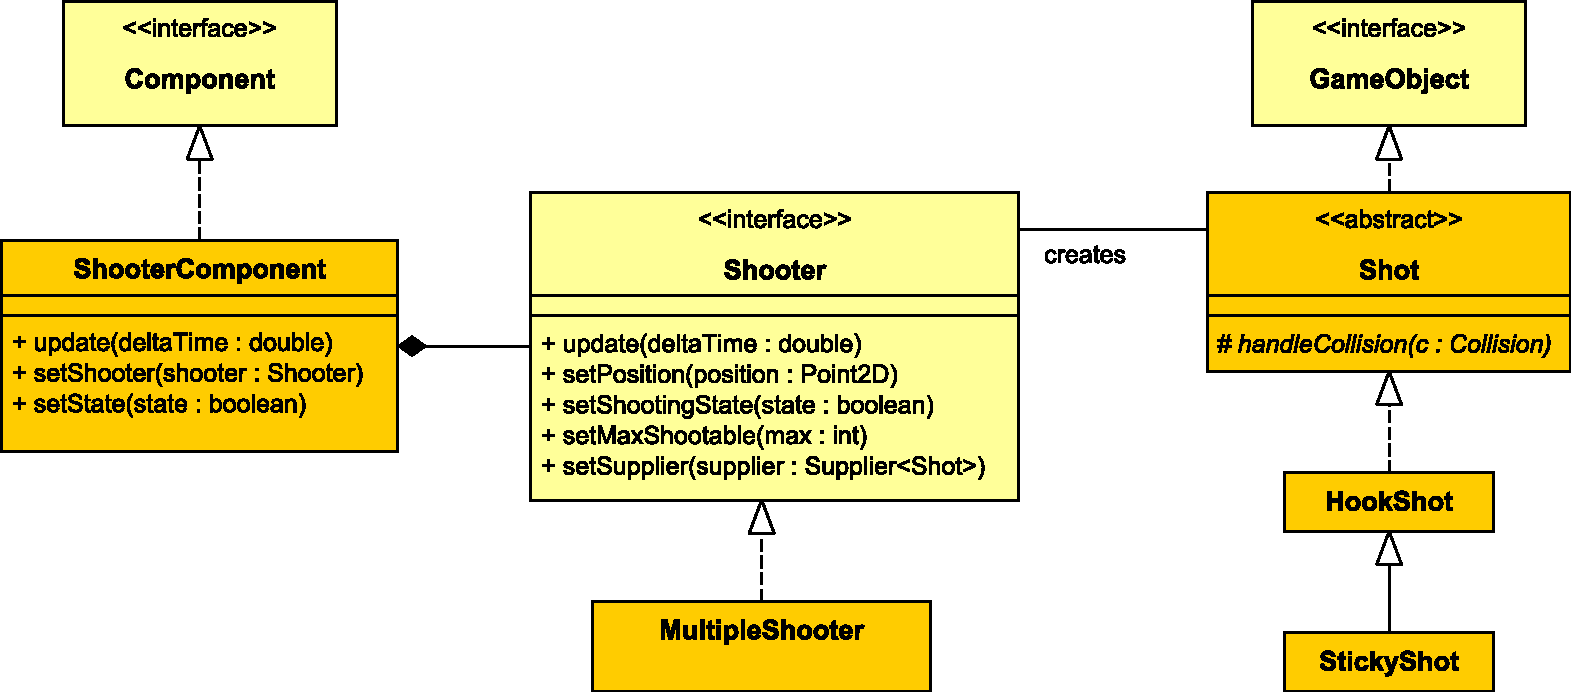
\includegraphics[width=\linewidth]{img/shooter}
\caption{Struttura del meccanismo di shooting in cui è visibile il pattern Bridge.}
\label{img:shooter}
\end{figure}

\subsubsection*{Power Rendering}

Per visualizzare l'azione dei TimedPower sullo schermo e fornire all'utente un segnale più evidente della fine imminente dell'azione di un determinato potere, rendendo così il gamePlay più facile, ho realizzato dei TimeableRenderer.

L'interfaccia Timeable rappresenta un qualsiasi oggetto dotato di una durata specifica nel tempo.
Questi oggetti sono in grado di segnalare ogni volta che il proprio contatore interno viene modificato tramite un evento e anche quando invece il tempo è completamente esaurito. 

I TimeableRenderer sono Renderer capace di autodistruggersi registrandosi all'evento di timeout, per questo motivo tengono un'instanza del CanvasDrawer in modo da potersi eliminare autonomamente dalla lista dei Renderer attivi. 

Per segnalare in modo evidente che il tempo si sta esaurendo ho deciso di creare una specializzazione dei TimeableRenderer in grado di "lampeggiare" (blink) e quindi di scegliere se essere renderizzati o meno a seconda del tempo rimanente.

\begin{figure}[H]
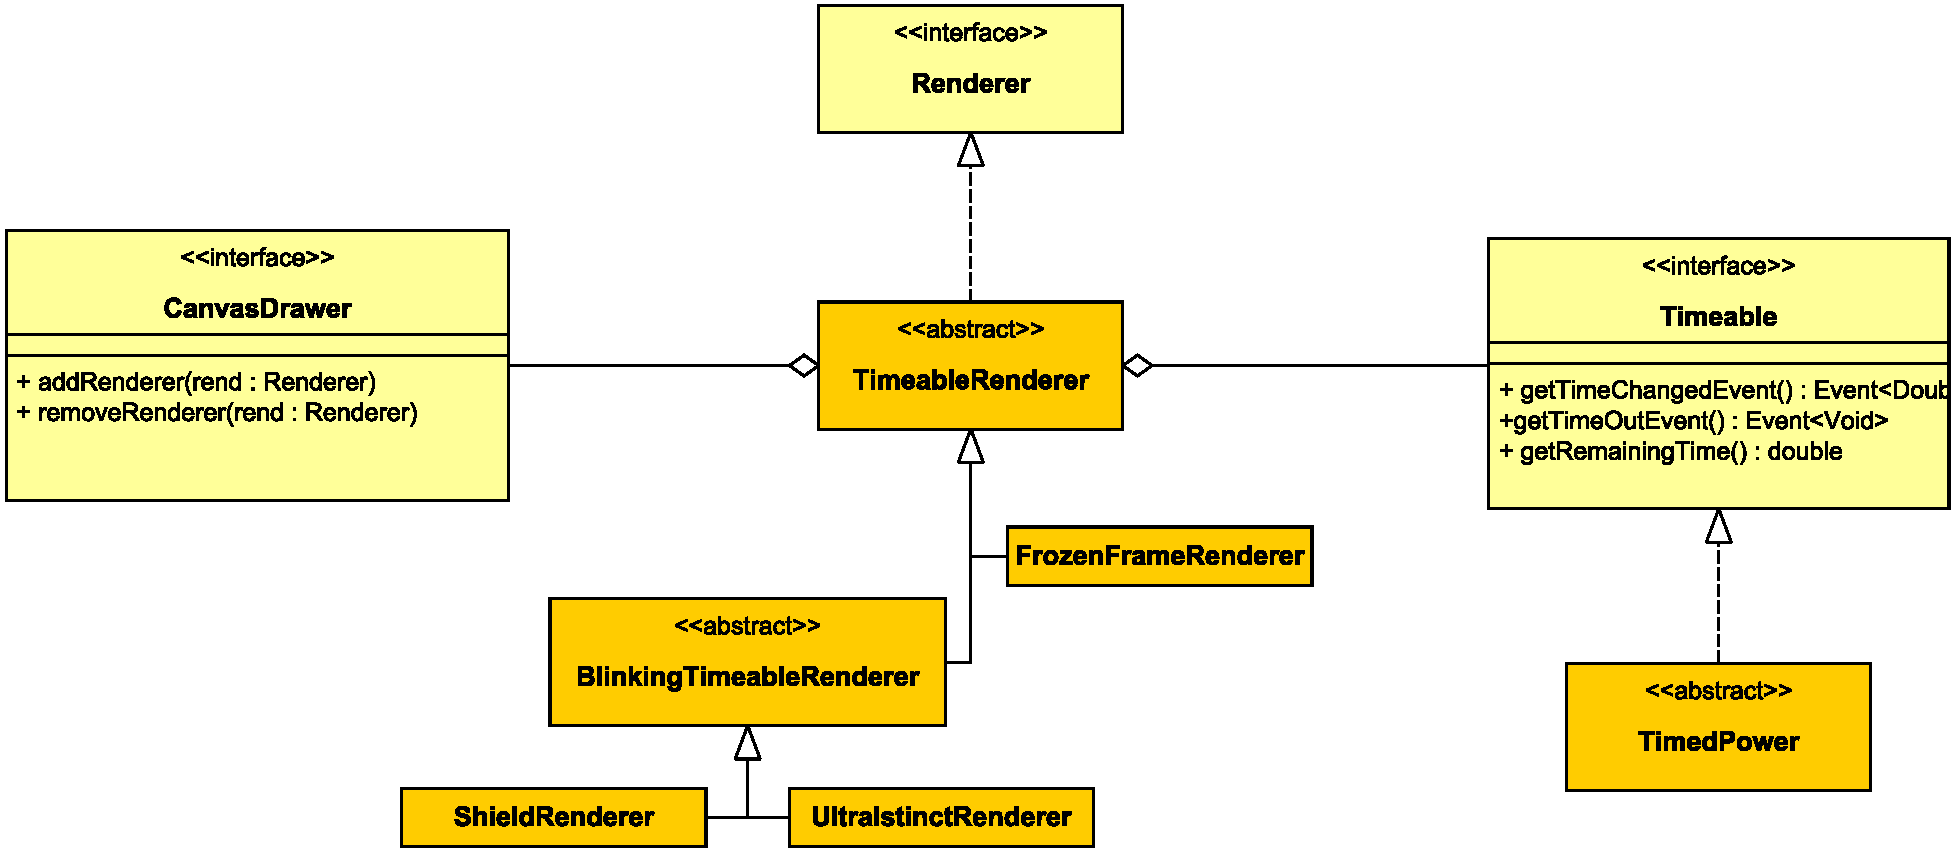
\includegraphics[width=\linewidth]{img/power_rendering}
\caption{Schema UML della struttura del rendering per i powers.}
\label{img:power_rendering}
\end{figure}

\subsubsection*{GameObjectVisitor}

Nella fase di sviluppo mi sono reso conto che spesso avevamo bisogno di operare azioni differenti a seconda del tipo di Gameobject pur non avendo un modo semplice per distinguerli.
Una soluzione sarebbe potuta essere aggiungere nuovi metodi all'interfaccia GameObject, ma sarebbe andato spesso in conflitto con l'architettura MVC.
Ho quindi deciso di riprogettare il codice per poter sfruttare il pattern \textbf{Visitor}.
In questo modo i GameObject possono accettare appunto un visitor che può modificare o interagire con l'oggetto ed eventualmente ritornare un valore. Come si può osservare in \Cref{img:visitor} l'interfaccia GameObjectVisitor 

Siccome in alcuni casi non era necessario eseguire operazioni per certi tipi di oggetto, abbiamo implementato anche una versione di base astratta del GameObjectVisitor, che implementa tutti metodi restituendo un valore di default.
In questo modo è necessario ridefinire solamente il comportamento per gli oggetti desiderati.

\begin{figure}[H]
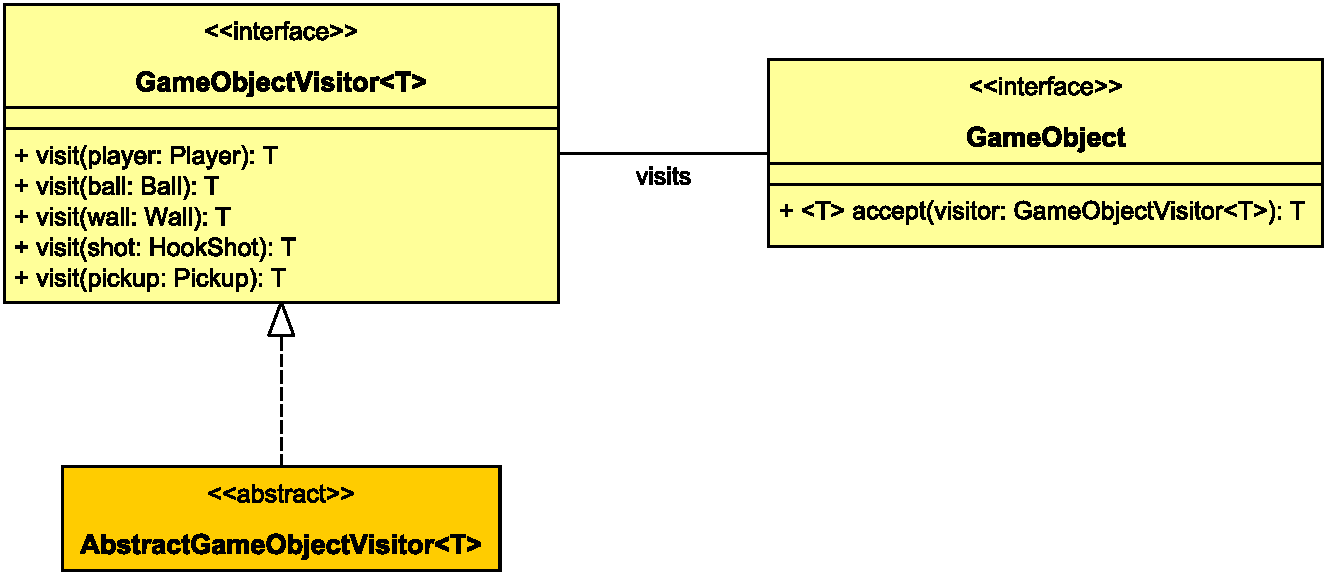
\includegraphics[width=\linewidth]{img/visitor}
\caption{Schema UML della struttura del pattern Visitor applicato ai GameObject.}
\label{img:visitor}
\end{figure}

\subsection*{Nicholas Ciarafoni}

\subsubsection*{Pickups e Powers}

Per la realizzazione del GameObject Pickup, ho subito fatto una differenza fra oggetto e potenziamento, creando a parte l'interfaccia Power che gestisce poi (con l'ausilio di altre classi) i vari potenziamenti che possono essere attivati sul Player e sulle Ball interne al Level corrente.
L'oggetto Pickup prende come parametro un Power che definisce il modo in cui lo stato del gioco viene modificato all'atto del raccoglimento.
All'interno dei Power sono state individuate due tipologie di potenziamento in delle classi astratte, una TimedPower per i potenziamenti che hanno un preciso tempo di vita e una volta terminato si disattivano, e InstantPower per quei potenziamenti che non hanno un tempo di vita limitato, ma persistono per tutta la durata del livello.
Per l'effettiva creazione dei power ho utilizzato il pattern creazionale \textbf{Static Factory}, con il metodo create(), che permette di creare un power in base al suo livello.
Per la creazione in game dei power, per rendere la logica di gioco inconsapevole di che tipo di utente è loggato e quali sono i livelli dei suoi power, ho utilizzato il pattern \textbf{Abstract Factory}, fornendo due implementazioni: una BasicPowerFactory, utilizzata per tutti gli utenti ospiti, che privi di registrazione, possono solamente giocare non avendo alcuna possibilità di aumentare e salvare i propri progressi di gioco.
La seconda invece UpgradePowerFactory è utilizzata per gli utenti registrati che possono aumentare i livelli di tutti i power spendendo dei Coins che automaticamente il giocatore guadagna passando i livelli.
L'utilizzo di questa struttura composta permette la possibile creazione di nuovi Powers futuri, riutilizzando più codice possibile evitandone quindi la superflua ripetizione.

\begin{figure}[H]
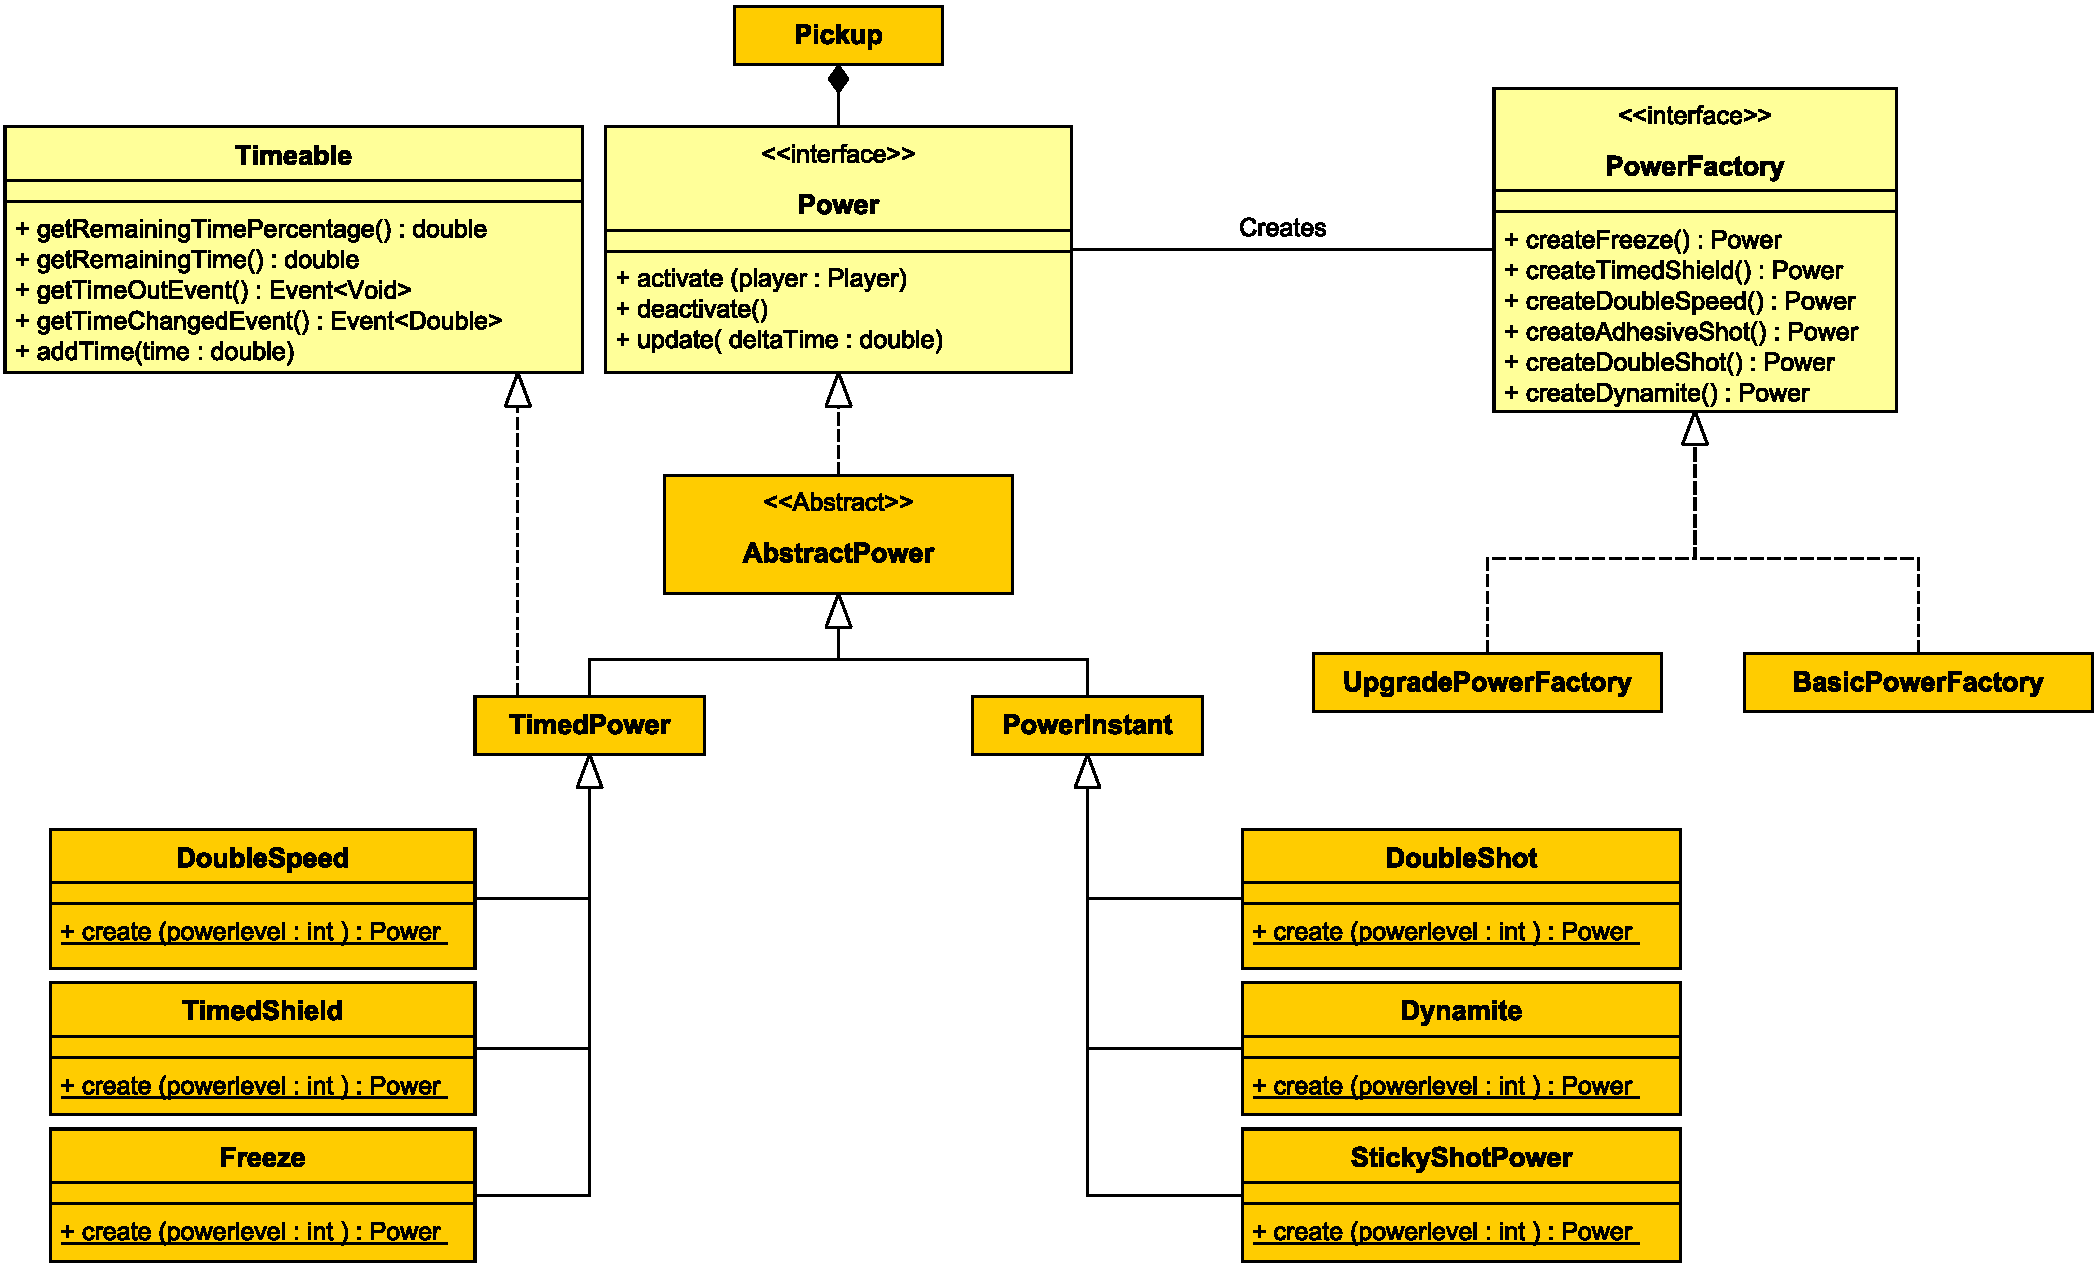
\includegraphics[width=\linewidth]{img/powers}
\caption{Schema UML che rappresenta i meccanismi utilizzati per Pickups e Powers.}
\label{img:powers}
\end{figure}

\subsubsection*{Leaderboard}
Per la gestione della Leaderboard ho creato un'interfaccia LeaderboardManager che fornisce 4 metodi rispettivamente per le fasi di caricamento e salvataggio dei dati nelle due rispettive modalità di gioco (TourMode e Survival).
L'implementazione concreta poi è svolta all'interno della classe FileSystemLeaderboardManager con relativa lettura e scrittura su file. In questo modo il Controller è ignaro di quale meccanismo si stia effettivamente utilizzando per mantenere la persistenza dei dati.
Per Il salvataggio dei record personali (LeaderboardRecord) sono state valutate 2 caratteristiche importanti: il punteggio (Score) e lo Stage raggiunto, che nella modalità Survival conta il numero di palle create, e nella modalità Tour conta invece il livello raggiunto sui 17 disponibili. 

\begin{figure}[H]
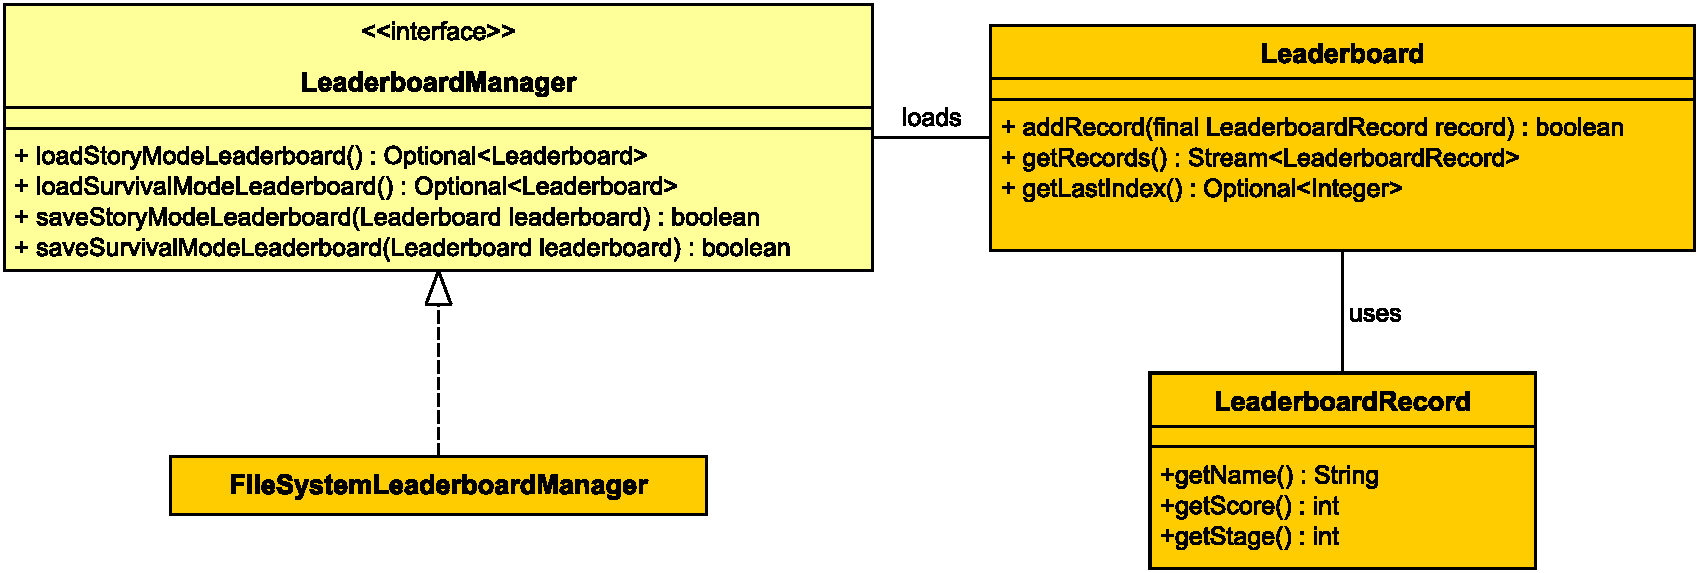
\includegraphics[width=\linewidth]{img/leaderboard}
\caption{Schema UML che mostra la gestione della leaderboard.}
\label{img:leaderboard}
\end{figure}

\subsection*{Francesco Dente}

\subsubsection*{Events}

Un elemento fondamentale della progettazione dell'applicazione è stata la modellazione del concetto di evento seguendo il pattern \textbf{Observer}.
In uno scenario così dinamico in cui lo stato del sistema cambia molto frequentemente, si intuisce chiaramente come la strategia di "polling" (interrogazione periodica) sia inefficacie.
Abbiamo dunque deciso di sfruttare questo pattern.

Il suo fulcro è l'interfaccia Event, che rappresenta un'avvenimento al quale uno o più listener (descritti dall'interfaccia EventHandler) possono interessarsi.
Ogni evento porta con se anche un tipo (T) relativo alle informazioni riguardanti l'avvenimento.

I metodi register() e unregister() permettono agli handler di iniziare o smettere di ascoltare l'evento stesso.
Dal momento della registrazione, ogni volta che l'evento viene innescato tutti i suoi osservatori vengono automaticamente notificati tramite il metodo handle().

La concretizzazione principale dell'interfaccia Event è EventSource, che contiene la logica per innescare l'evento e notificarne i gestori.
Ho deciso di non rendere disponibile il metodo trigger() tramite l'interfaccia per non dare la possibilità ad oggetti esterni al possessore dell'evento di innescarlo.
In questo modo solo la reale sorgente dell'evento ne ha la possibilità.

L'implementazione CompositeEvent rende invece possibile trattare più eventi "simili" come se fossero uno solo, seguendo appunto il pattern \textbf{Composite}.

Infine il NullEvent rappresenta un evento che, non potendo essere attivato, ignora semplicemente le richieste di register() e unregister().
La necessità di questa classe è dovuta alla presenza nel progetto di interfacce che richiedono la presenza di un certo evento.
Capita però in alcuni casi che certe implementazioni non siano realmente sorgenti per quel particolare evento.
In questo modo è possibile restituire comunque un oggetto compatibile con l'interfaccia Event anche se fasullo.

\begin{figure}[H]
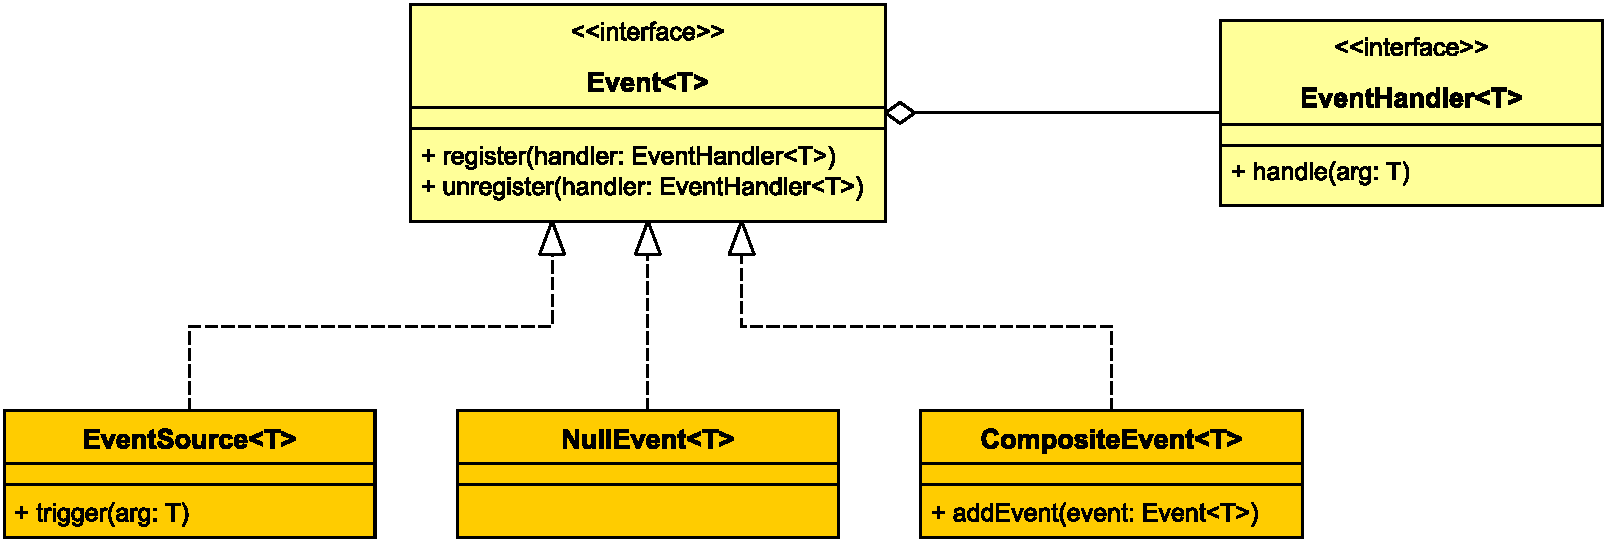
\includegraphics[width=\linewidth]{img/events}
\caption{Schema UML della struttura degli eventi.}
\label{img:events}
\end{figure}

\subsubsection*{Collisions}

Una parte di cui mi sono occupato è stata la rilevazione delle collisioni.
Nella scena sono infatti presenti entità che devono poter reagire non appena entrano in contatto con altri oggetti, ognuna secondo regole diverse.

Un'unità che ha la capacità di collidere viene rappresentata dall'interfaccia Collidable ed è dotata di una posizione e di una forma.
La gestione globale delle collisioni è invece affidata al CollisionManager che, venendo periodicamente richiamato dal Level, verifica quali coppie di Collidable sono in contatto in un determinato momento.
Ogni coppia viene quindi notificata tramite il metodo notifyCollision(), dove riceve informazioni riguardanti l'urto.
É compito del Collidable a questo punto informare chi è interessato tramite un evento.
Questo permette ai diversi GameObject che possiedono il Collidable di reagire in modo diverso alla collisione.

Sfruttando l'impalcatura fornita dai Component e il loro legame con i GameObject, ho pensato di implementare l'interfaccia Collidable tramite il CollisionComponent, permettendo facile accesso all'evento di collisione tramite l'interfaccia di GameObject.

\begin{figure}[H]
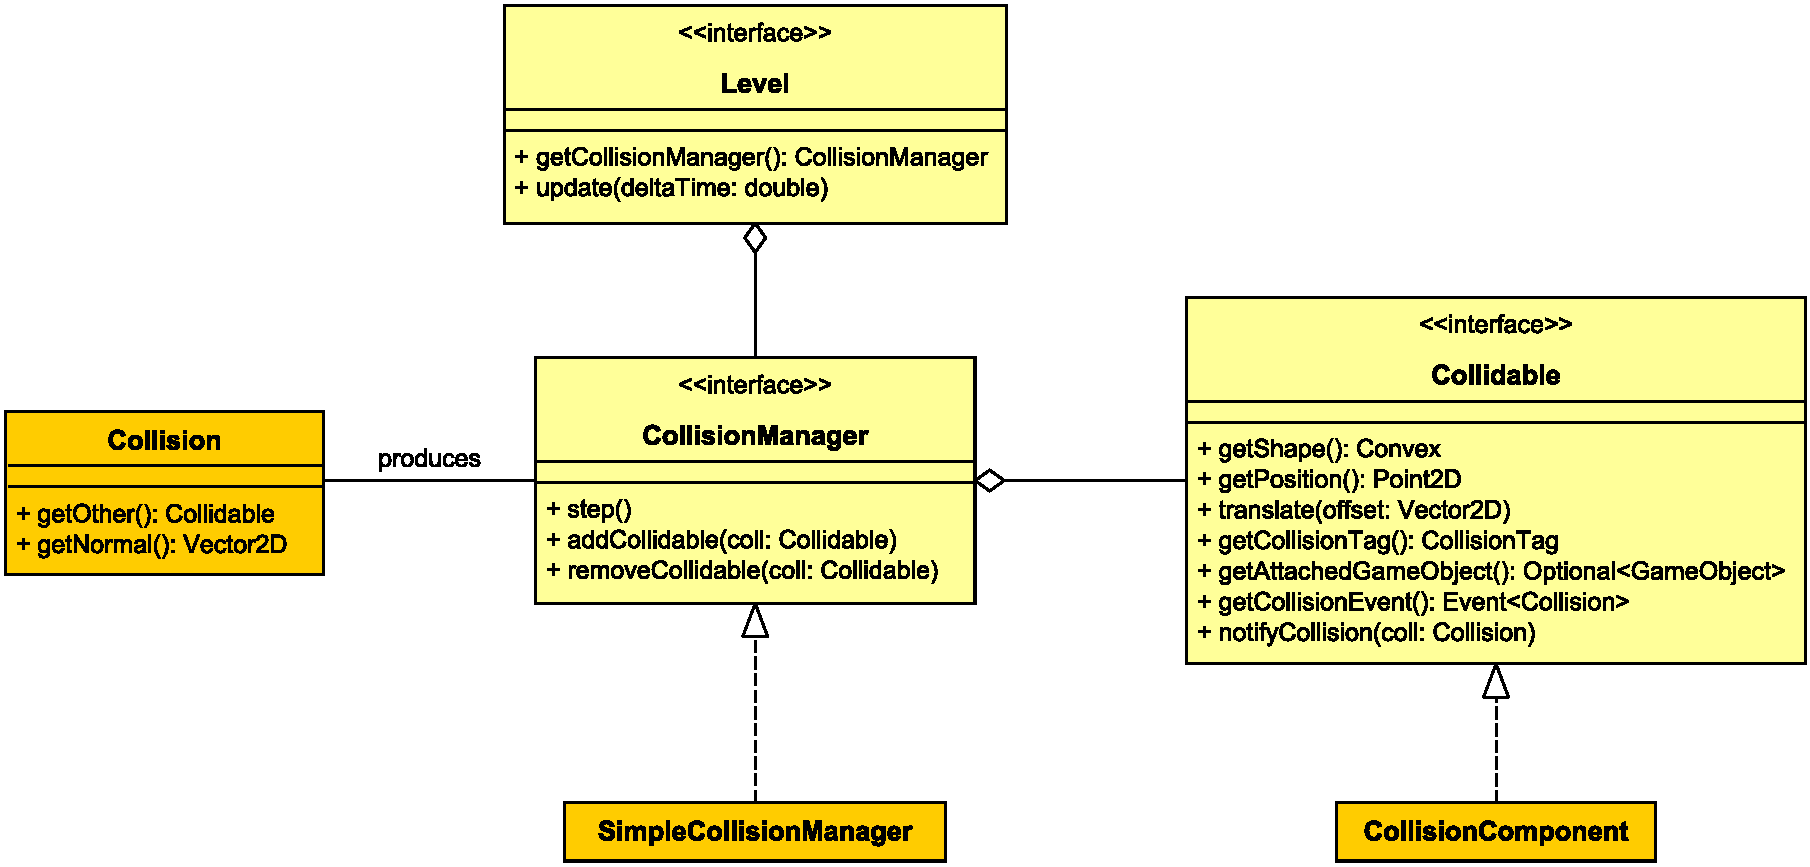
\includegraphics[width=\linewidth]{img/collisions}
\caption{Schema UML che descrive l'architettura per la gestione delle collisioni.}
\label{img:collisions}
\end{figure}

\subsubsection*{Rendering}

L'attore principale nella gestione del rendering è l'interfaccia Renderer, che non è altro che un'oggetto che sa come disegnarsi sullo schermo tramite il metodo render().
Questo concetto viene poi esteso nell'interfaccia Sprite, che aggiunge concetti come posizionamento e dimensioni.
Entrambe le interfacce sono state inizialmente estese da classi astratte (GenericRenderer e GenericSprite) che fornissero un'implementazione di base indipendente dal motore grafico per minimizzare le riscritture nell'ipotesi di un futuro cambio di framework.
In seguito ho fornito una prima implementazione concreta per Sprite che si basa su JavaFX.

A questo punto ho deciso di concentrarmi sul rendering dei GameObject, cercando una soluzione che restasse totalmente indipendente dal gestore grafico.
Per fare ciò ho creato una classe astratta GameObjectRenderer, che fa da wrapper sia per uno Sprite, utilizzato per l'effettivo disegno, che per un GameObject.
Ogni specializzazione gestirà in modo diverso la grafica per un particolare oggetto.

Per coordinare la molteplicità di oggetti da disegnare, i Renderer vengono gestiti da un CanvasDrawer, che espone all'esterno una \textbf{Abstract Factory} per la loro creazione (RendererFactory).
Anche in questo caso ho voluto impostare un'architettura che risentisse in minima parte dei possibili cambiamenti futuri, fornendo alcune implementazioni base, specializzandole poi in quelle legate a JavaFX.

\begin{figure}[H]
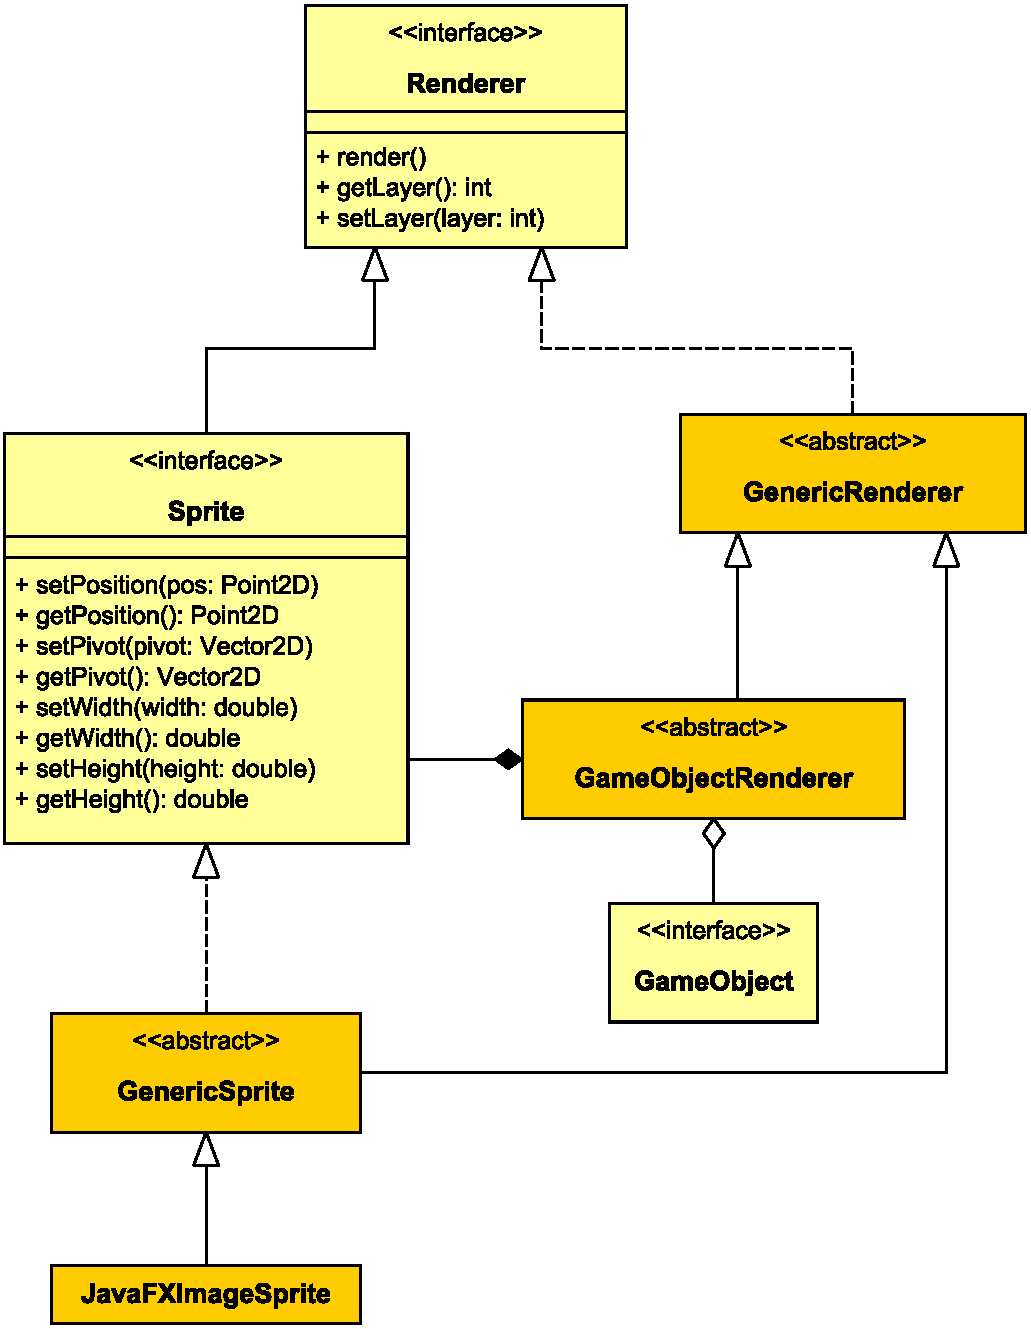
\includegraphics[width=\linewidth]{img/renderers}
\caption{Schema UML che mette in evidenza la gerarchia alla base della gestione del Rendering.}
\label{img:renderers}
\end{figure}

\begin{figure}[H]
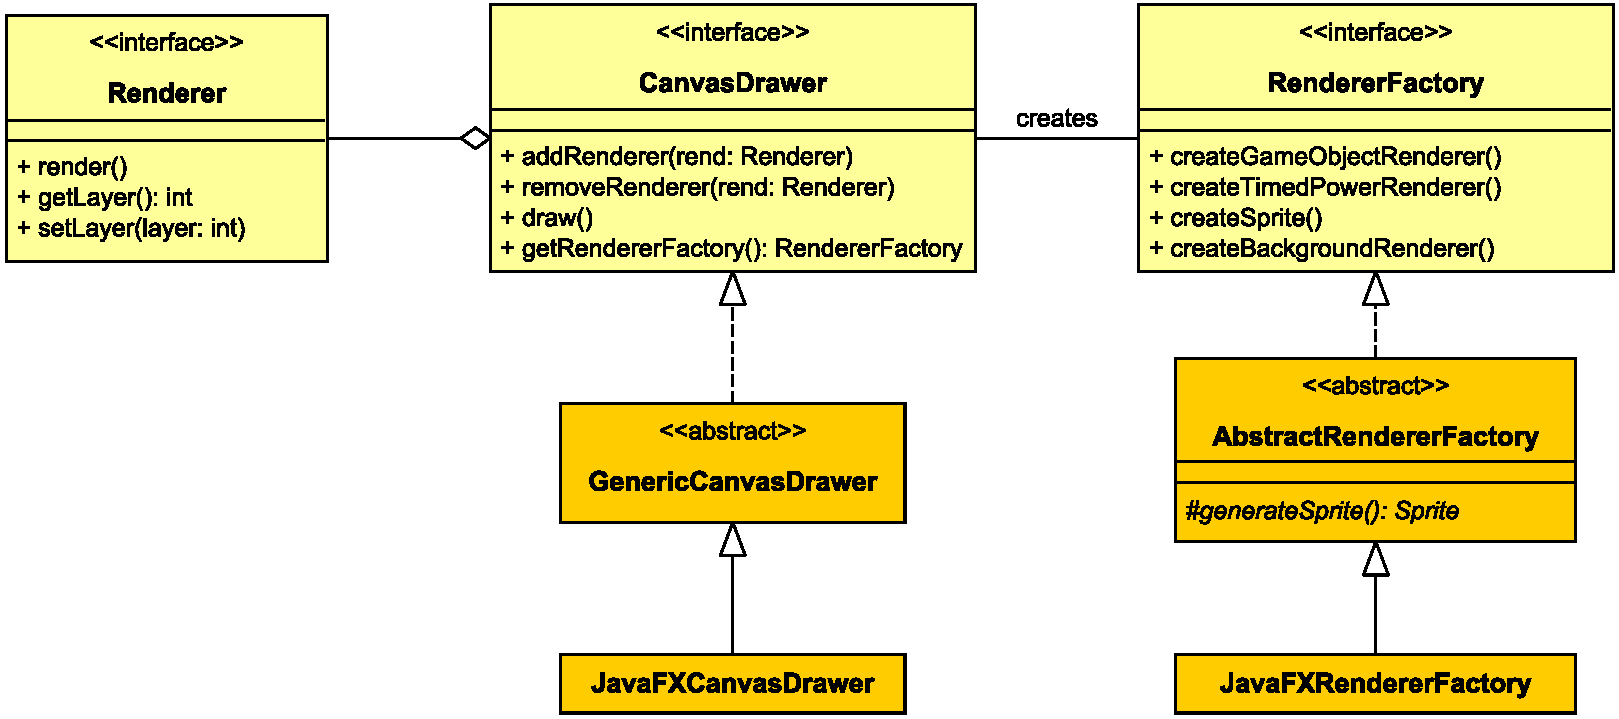
\includegraphics[width=\linewidth]{img/canvas_drawer}
\caption{Schema UML che mostra l'interazione tra Renderers e CanvasDrawer per mezzo della RendererFactory.}
\label{img:canvas_drawer}
\end{figure}

\subsubsection*{Level Decorators}

In seguito all'analisi delle funzionalità dell'applicazione, sono emerse feature che hanno reso il concetto di livello molto difficile da racchiudere in una sola classe.
Infatti la molteplicità di comportamenti diversi che il livello avrebbe dovuto avere, insieme alla necessità di poterli modificarli in base alle scelta della modalità, mi ha portato all'utilizzo del pattern \textbf{Decorator}.
Questa scelta ci ha permesso di comporre dinamicamente le funzionalità del gioco sulla base delle scelte dell'utente, senza creare classi che aggregassero insieme troppi concetti diventando difficilmente maneggiabili.

Abbiamo quindi creato un'implementazione basilare per un livello che contiene esclusivamente la logica core.
Dopodichè ho creato un'astrazione di decoratore dalla quale ho poi derivato una specializzazione per ogni feature aggiuntiva possibile, come la gestione del tempo, dello spawn di pickup, ecc.

A mano a mano che procedevamo però, ci rendevamo conto che spesso l'aggiunta di comportamenti richiedeva un cambiamento al modo di creare GameObject, rendendo quindi necessario modificare dinamicamente anche il comportamento della factory di GameObject.
Ho quindi deciso di estendere il pattern anche alla Factory, in modo che ogni LevelDecorator potesse decorare a sua volta la factory restituita dal livello decorato.

Questa impalcatura ci permetterà anche in futuro di aggiungere sia nuove modalità, sia nuove feature senza cambiare troppo la struttura del resto del modello.

\begin{figure}[H]
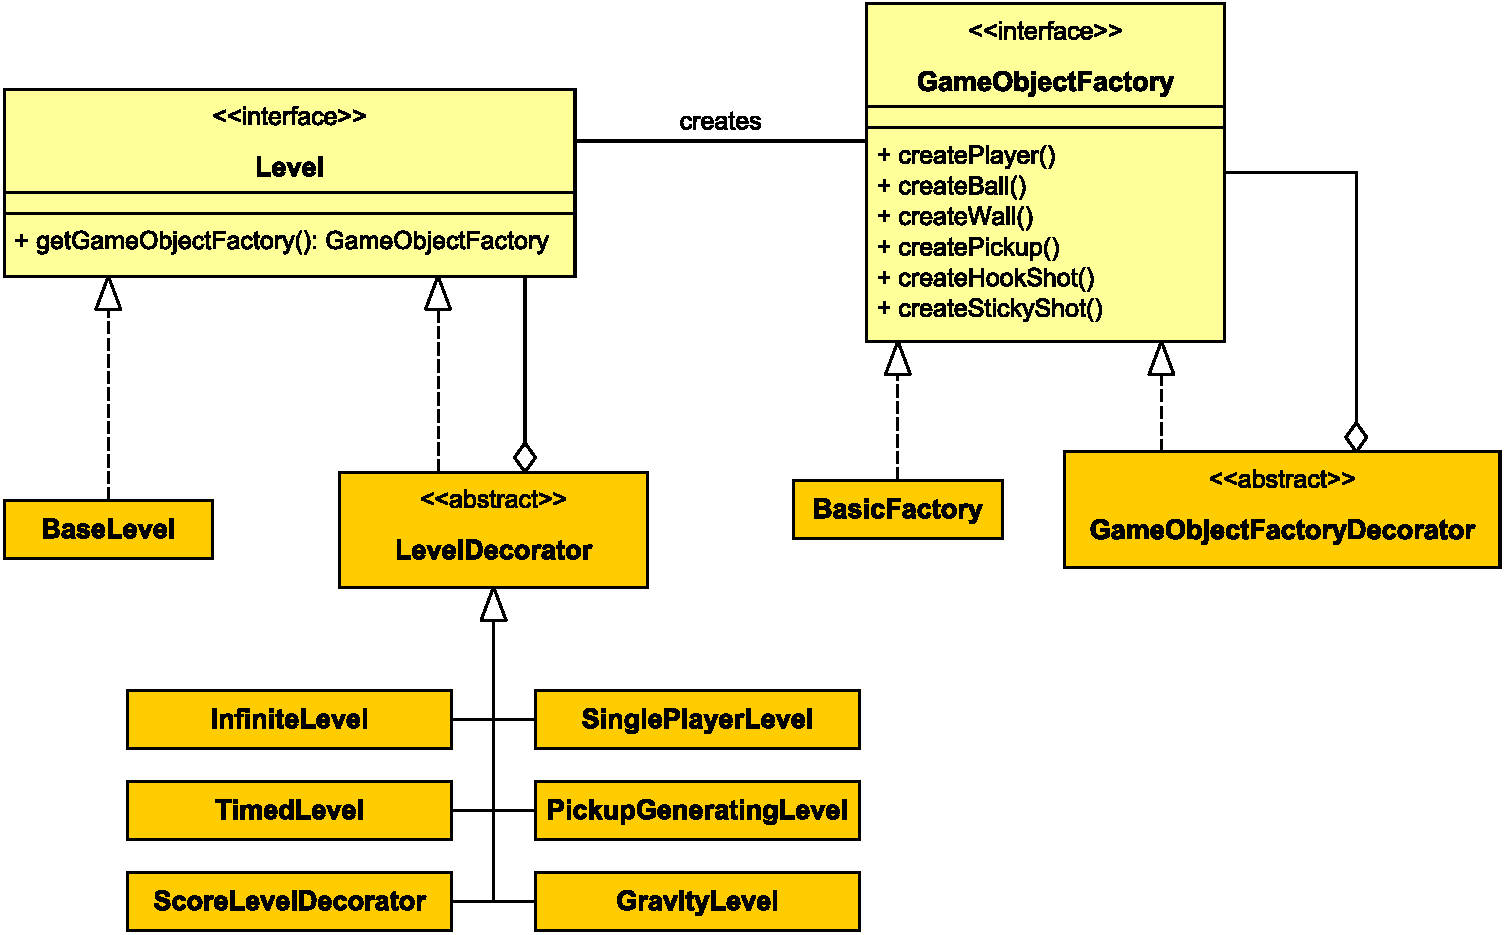
\includegraphics[width=\linewidth]{img/decorator}
\caption{Schema UML che mostra l'utilizzo del pattern Decorator per le interfacce Level e GameObjectFactory.}
\label{img:decorator}
\end{figure}

\subsection*{Lorenzo Menghini}

\subsubsection*{Component}

Dopo un'analisi dettagliata dei principali oggetti presenti nel gioco abbiamo delineato delle azioni comuni che questi oggetti potevano compiere come collidere, muoversi, ricevere input dall'utente, ed abbiamo strutturato queste capacità in components che sono paragonabili a pezzi di un motore.

Questi si interfacciano con i GameObject distribuendo meglio i compiti di quest'ultimi e prendendosi la responsabilità di eseguire azioni su di essi.
La struttura favorisce riuso di codice poichè, essendo modulari, possono essere applicati ad ogni tipo di oggetto ed essendo indipendenti la modifica di parametri (ad esempio la modalità di movimento) va solamente applicata al singolo component invece che ad ogni oggetto interessato.

La classe astratta AbstractComponent delinea azioni comuni a tutte le sottoclassi come ad esempio l'abilitazione o disabilitazione del component stesso a seconda delle necessità durante l'esecuzione dell'applicazione; lasciando l'implementazione di alcuni di essi vuota ci permette di personalizzare ogni component in modo differente e funzionale.

\begin{figure}[H]
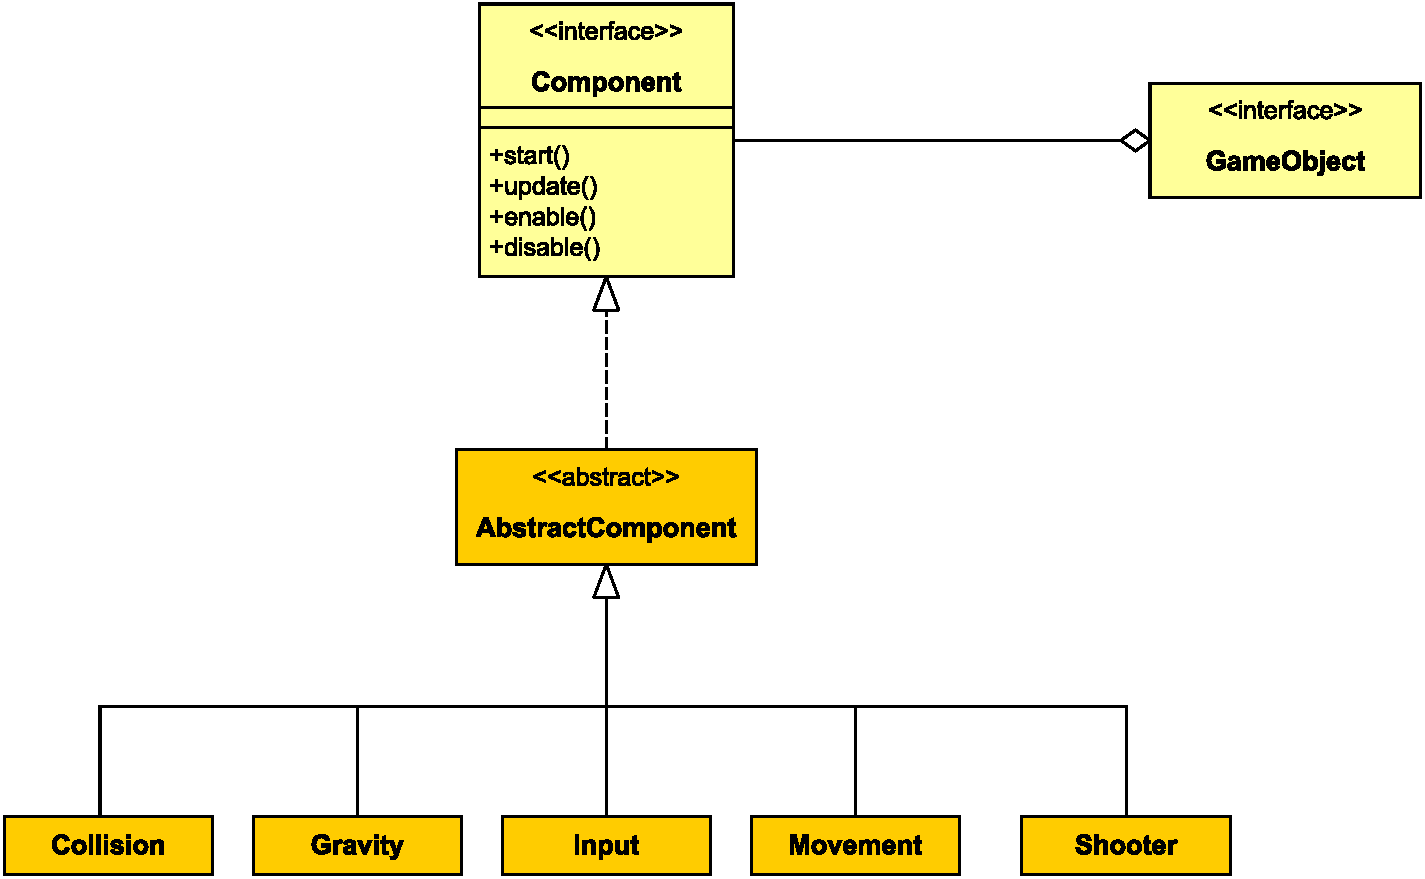
\includegraphics[width=\linewidth]{img/component}
\caption{Schema UML che illustra l'impalcatura generale dei Component}
\label{img:component}
\end{figure}

\subsubsection*{Input}

La gestione dell'input dall'utente è una parte fondamentale del software che coinvolge gran parte del progetto toccando le tre macro suddivisioni quali Controller, View e Model.
La struttura principale è a carico dell'InputController che si occupa di tenere immagazzinati i valori delle variabili di gioco (possibilità di sparo o cambi di direzione).

Per permettere la manipolazione di questi valori e allo stesso tempo proteggerne il contenuto, ho scelto di creare due distinte interfacce per differenziare i compiti di lettura o scrittura: il Model deve poter leggere i dati senza poterli modificare mentre la scrittura deve avvenire dall'esterno.
Alla cattura di un comando da parte dell'utente la View si occupa di invocare la sendCommand sul controller che aggiungerà a sua volta il comando catturato tra quelli da processare nel GameLoop.

Il GameLoop essendo l'unico ad avere l'accesso in scrittura all'InputController è responsabile di modificarne il contenuto coerentemente con il comando processato.
Ad ogni update l'InputComponent ha il compito di leggere ed interpretare i valori dall'InputReader e modificare i parametri del GameObject a cui appartiene.

\begin{figure}[H]
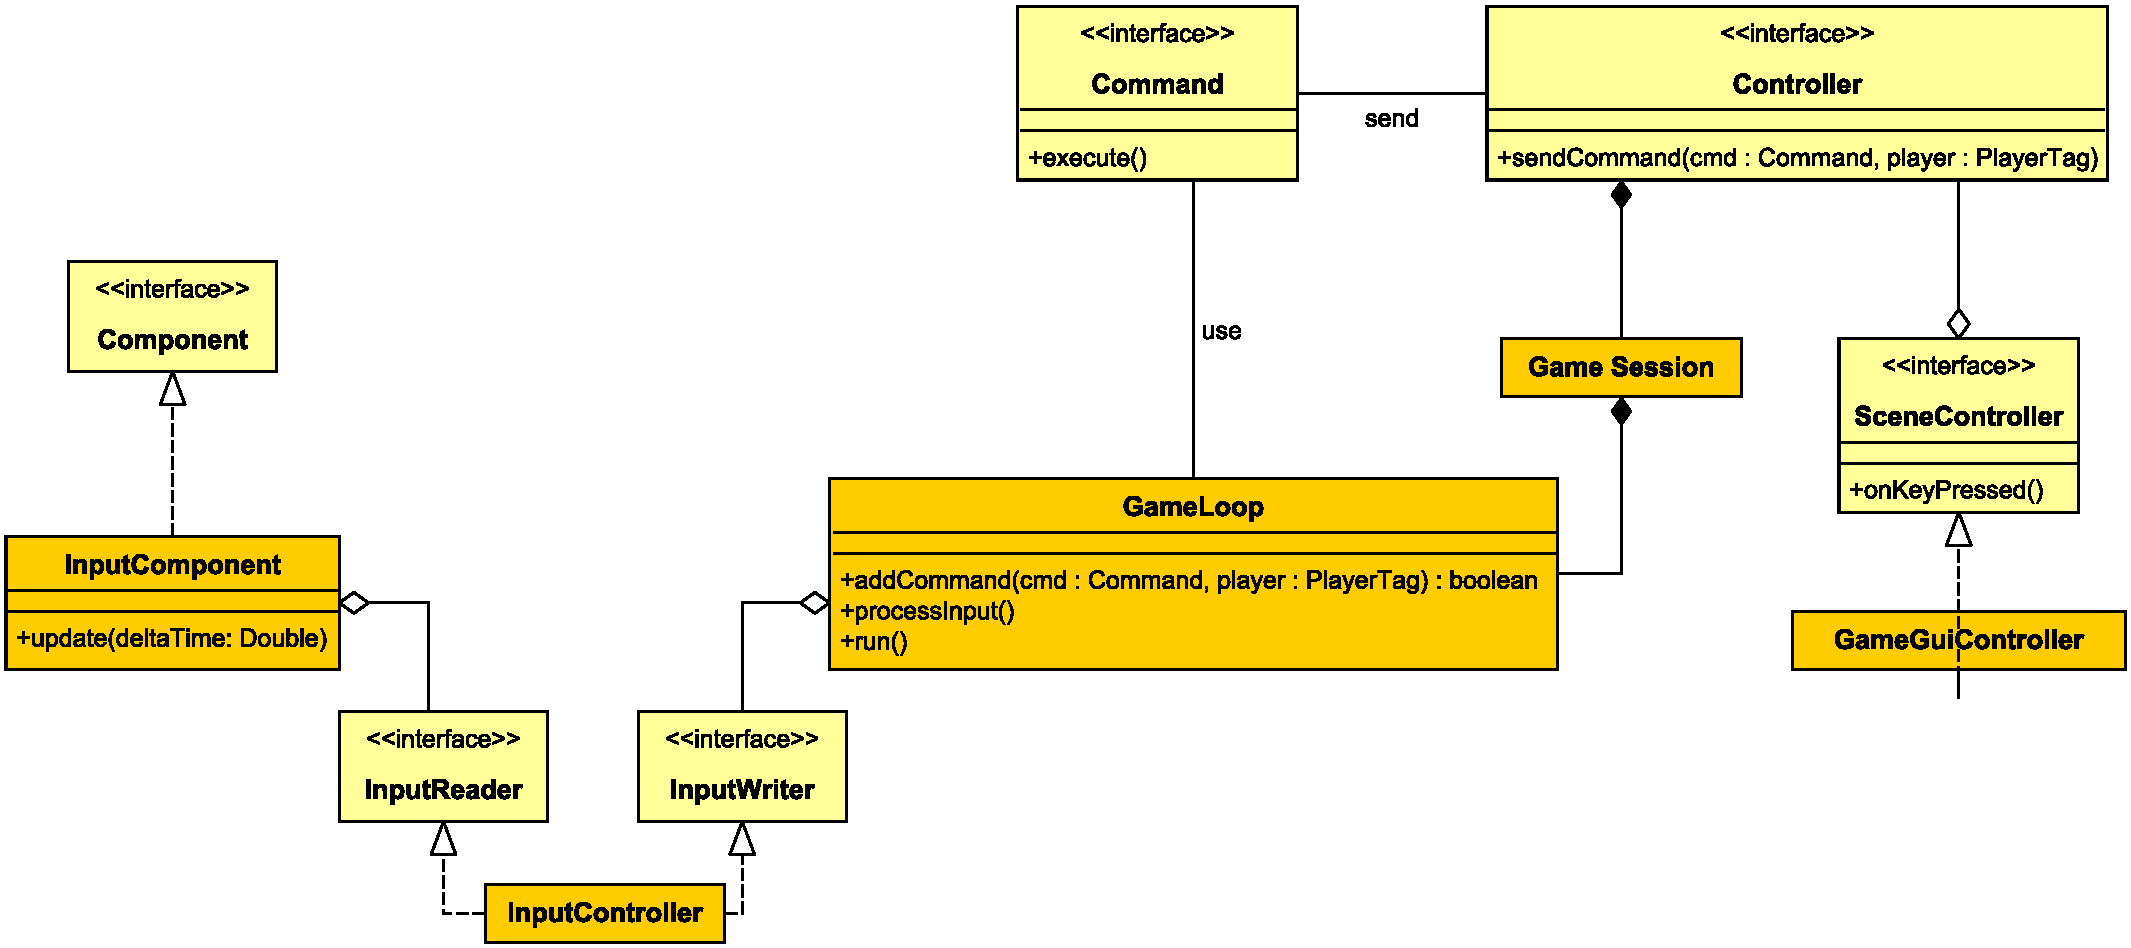
\includegraphics[width=\linewidth]{img/input}
\caption{Schema UML che spiega il collegamento effettuato per gestire l'Input trasversalmente tra il Model la View e il Controller}
\label{img:input}
\end{figure}

\subsubsection*{GameSession}

La GameSession è una parte fulcro del progetto poichè mette in comunicazione il Controller con la view e il model, permetendo il passaggio di informazioni in modo protetto.

Abbiamo specializzato il lavoro di questa sezione in due modalità differenti a seconda della modalità di gioco (Survival o StoryMode); 
La suddivisione si è resa necessaria per via delle notevoli differenze tra le due modalità di gioco: per citarne alcune il numero di vite, il conteggo dello stage (nella StoryMode si riferisce al livello attuale mentre nella Survial al numero di Balls distrutte) o anche per il semplice fatto che nella Survival non esiste un livello successivo.
Queste due parti si occupano inoltre di ricevere informazioni di gioco alla fine di ogni livello e di aggiornare di conseguenza la view che provvederà poi ad interfacciarsi con l'utente.
Come citato sopra sono responsabili di verificare la presenza di un nuovo livello possibile e di far agire il LevelLoader per provvedere al caricamento dei dati necessari.

\begin{figure}[H]
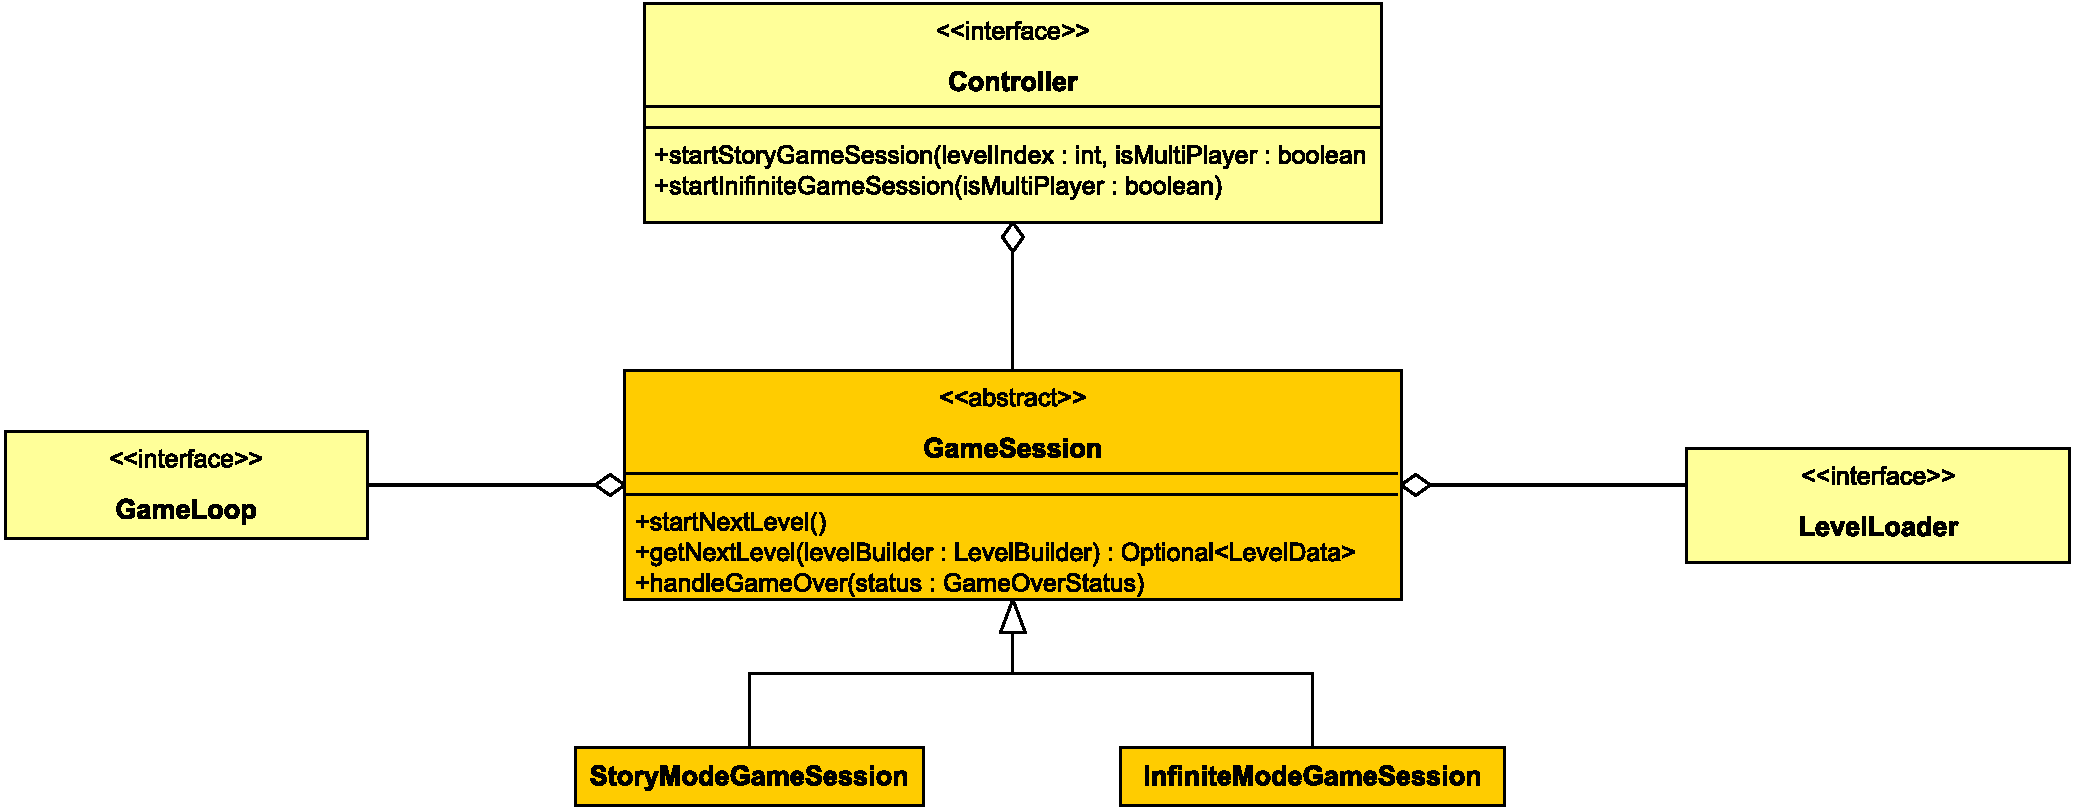
\includegraphics[width=\linewidth]{img/gamesession}
\caption{Schema UML che spiega il collegamento effettuato per gestire l'Input trasversalmente tra il Model la View e il Controller}
\label{img:gamesession}
\end{figure}

\subsubsection*{Loader}
Questa sezione del progetto è responsabile del caricamento da file (formato .xml) dei livelli e della decorazione di quest'ultimi attraverso l'inserimento delle proprietà e oggetti di gioco (Balls, Walls, ecc.).

Viene utilizziato all'avvio della scena di gioco dal controller per inizializzare la partita (startStoryModeSession/Survival), questo ha come compito quello di produrre un LevelData che contiene tutte le informazione necessarie per la costruzione.
\begin{figure}[H]
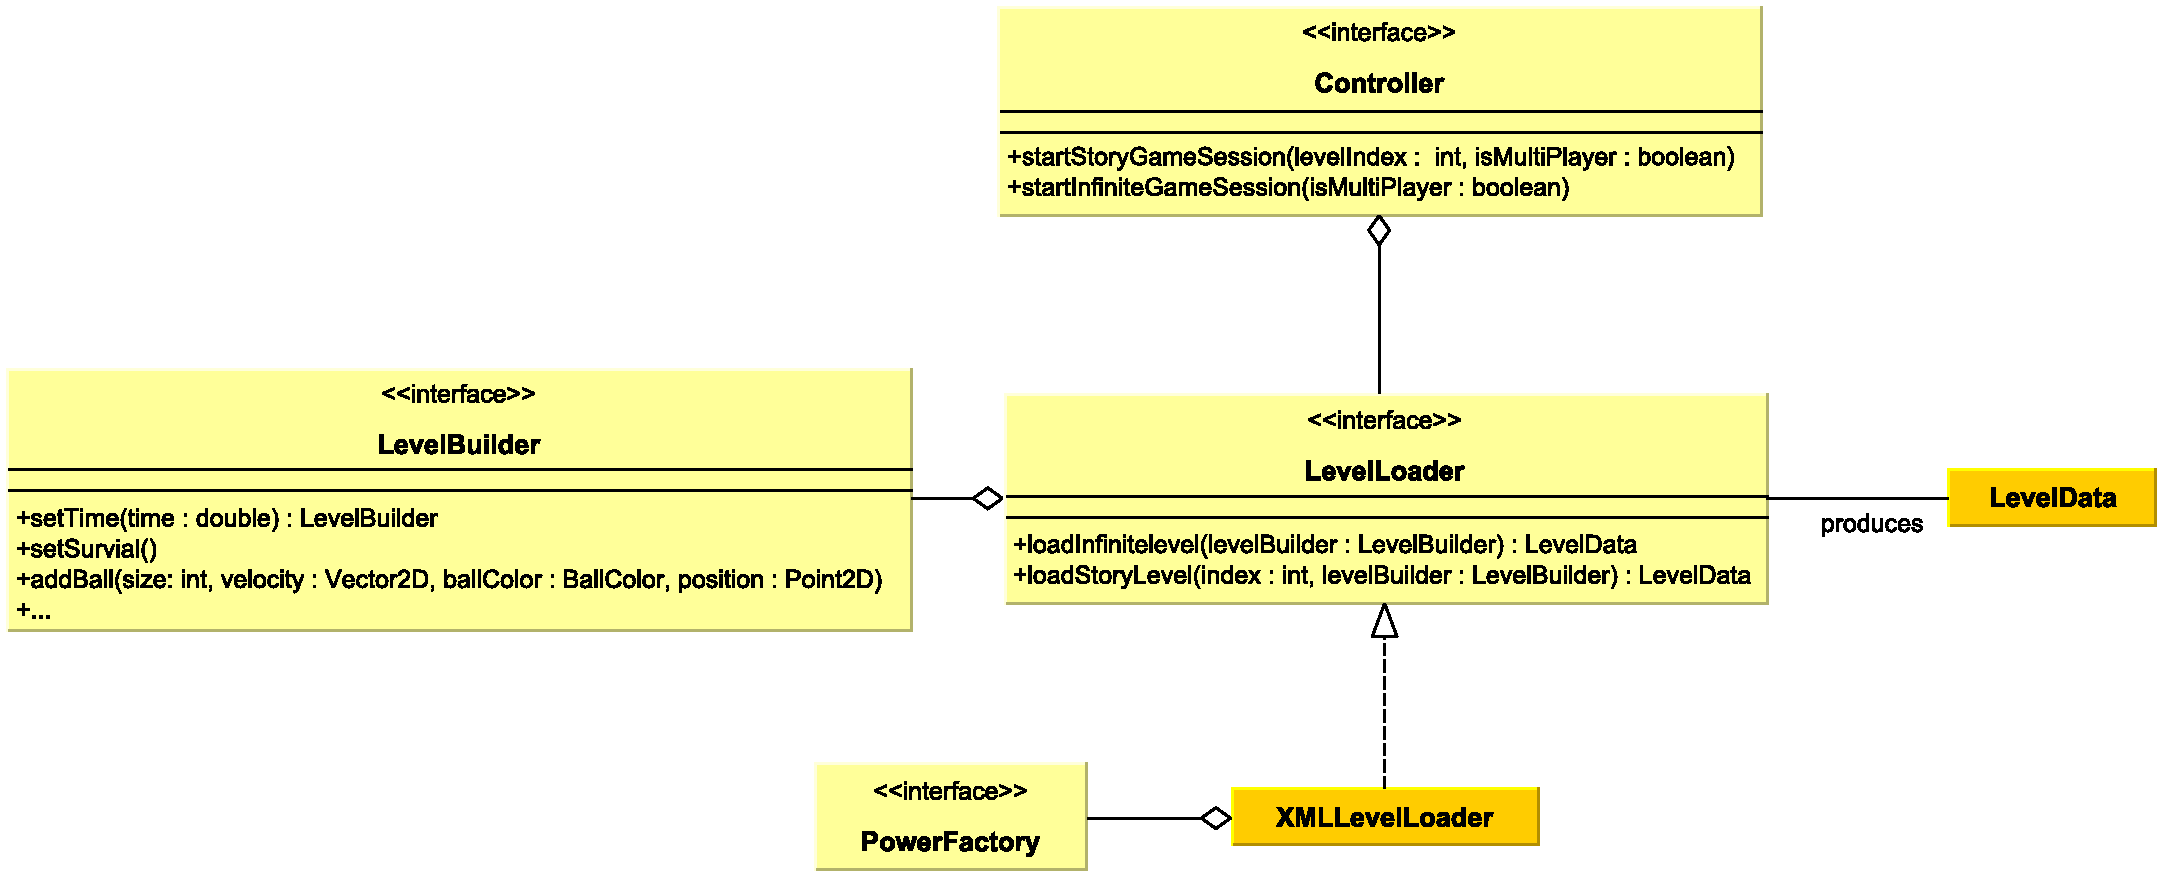
\includegraphics[width=\linewidth]{img/loader}
\caption{Schema UML che mostra la struttura del Loader in collegamento alla GameSession}
\label{img:loader}
\end{figure}


\subsection*{Francesca Tonetti}
\subsubsection*{Level Builder}
L'interfaccia LevelBuilder è realizzata seguendo il pattern di progettazione Builder.
Questo tipo di implementazione permette di gestire il problema della costruzione di un oggetto complesso come il Level, in modo che il processo di costruzione possa creare diverse rappresentazioni.

Le decorazioni di un livello sono così gestite unicamente dal builder e non dal codice client richiamando una struttura lazy, come specifica il nome della classe implementativa LazyLevelBuilder, poiché si deve seguire unicamente un certo ordine nelle operazioni e devono essere eseguite solo una volta che si hanno tutti i dati. 
La creazione di questa stessa interfaccia riporta uno stile fluent, infatti tutti i metodi di cui è composta restituiscono il LevelBuilder stesso.

\begin{figure}[H]
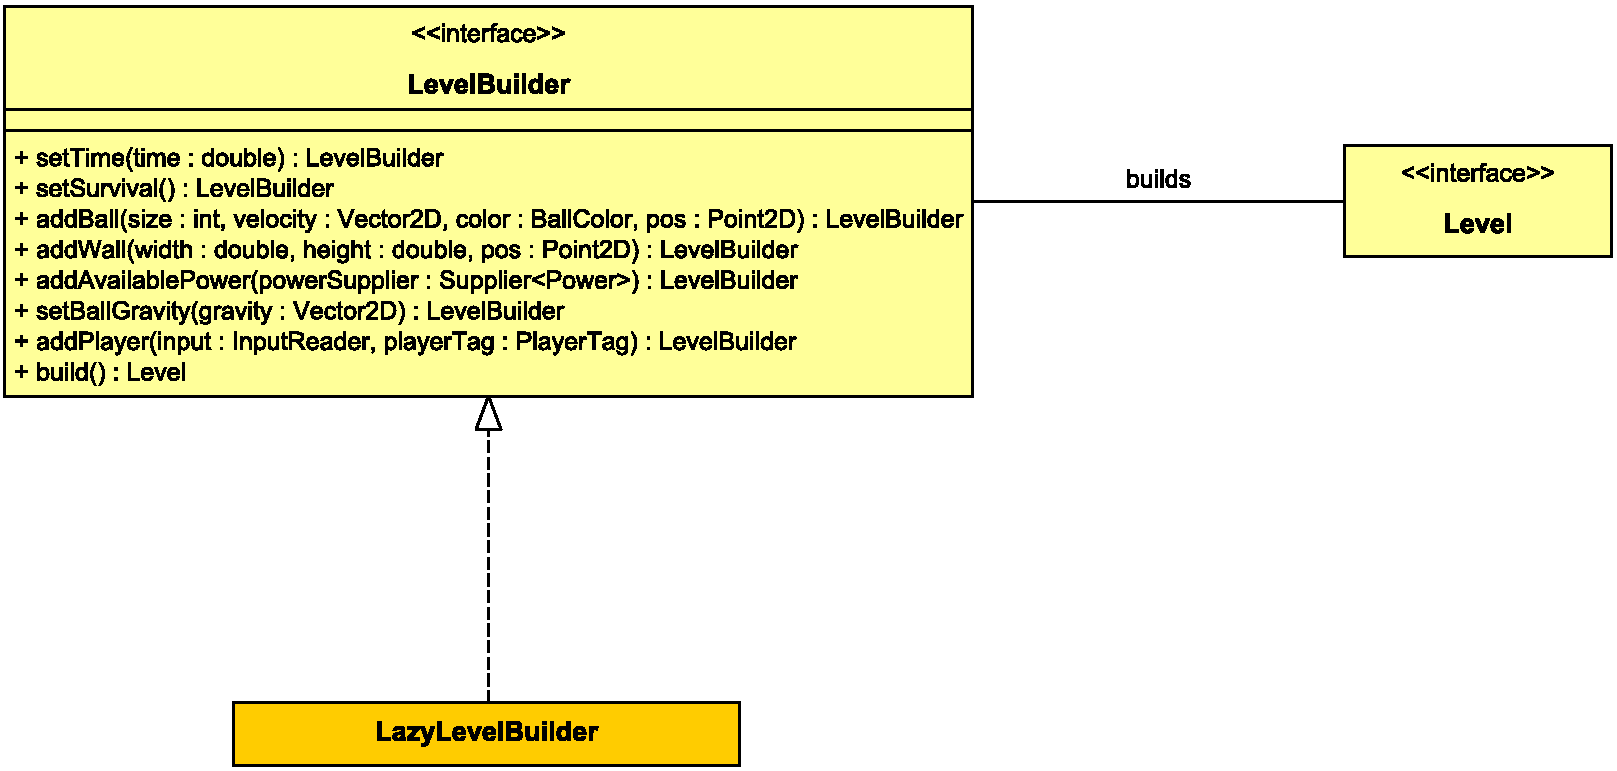
\includegraphics[width=\linewidth]{img/levelbuilder}
\caption{Schema UML che mostra la struttura del LevelBuilder}
\label{img:builder}
\end{figure}

\subsubsection*{User}
La classe User rappresenta il profilo di un utente a cui è associato un login con password per far si che ad ogni sessione di gioco i dati vengano conservati in maniera persistente, sicura e per permettere inoltre all'utente stesso di potenziare i propri power nell'ascesa ai livelli.
La creazione di un nuovo oggetto User ho deciso di affidarla allo UserManager dell'applicazione che viene a sua volta invocato dal Controller per effettuare la registrazione ed il login dell'utente.

I metodi fondamentali che compongono l'interfaccia UserManager riguardano il login() ed registerUser(), per questo ho scelto di dichiararli opzionali poiché rappresentano tipi di operazioni che possono talvolta non andare a buon fine. 
Il meccanismo di salvataggio è automatico in quanto lo User notifica il Controller tramite lo userModifiedEvent, innescando la riscrittura su file ogni qualvolta avviene una variazione dei dati, anche in questo caso nell'interfaccia UserManager ho pensato di dichiarare booleano il tipo di ritorno del metodo saveUser() che mostrerà true o false in base al terminazione corretta o viceversa.

All'interno della classe User si sviluppa tutta la logica di conversione dei punti accumulati dall'utente in punti esperienza, necessari per guadagnare monete ed aumentare il livello del proprio rank e poter così potenziare i power. Tale logica applicativa fa sì che un utente con punteggi più elevati possa ricevere ricompense migliori a mano a mano che si raggiungono i livelli più alti del gioco.

\begin{figure}[H]
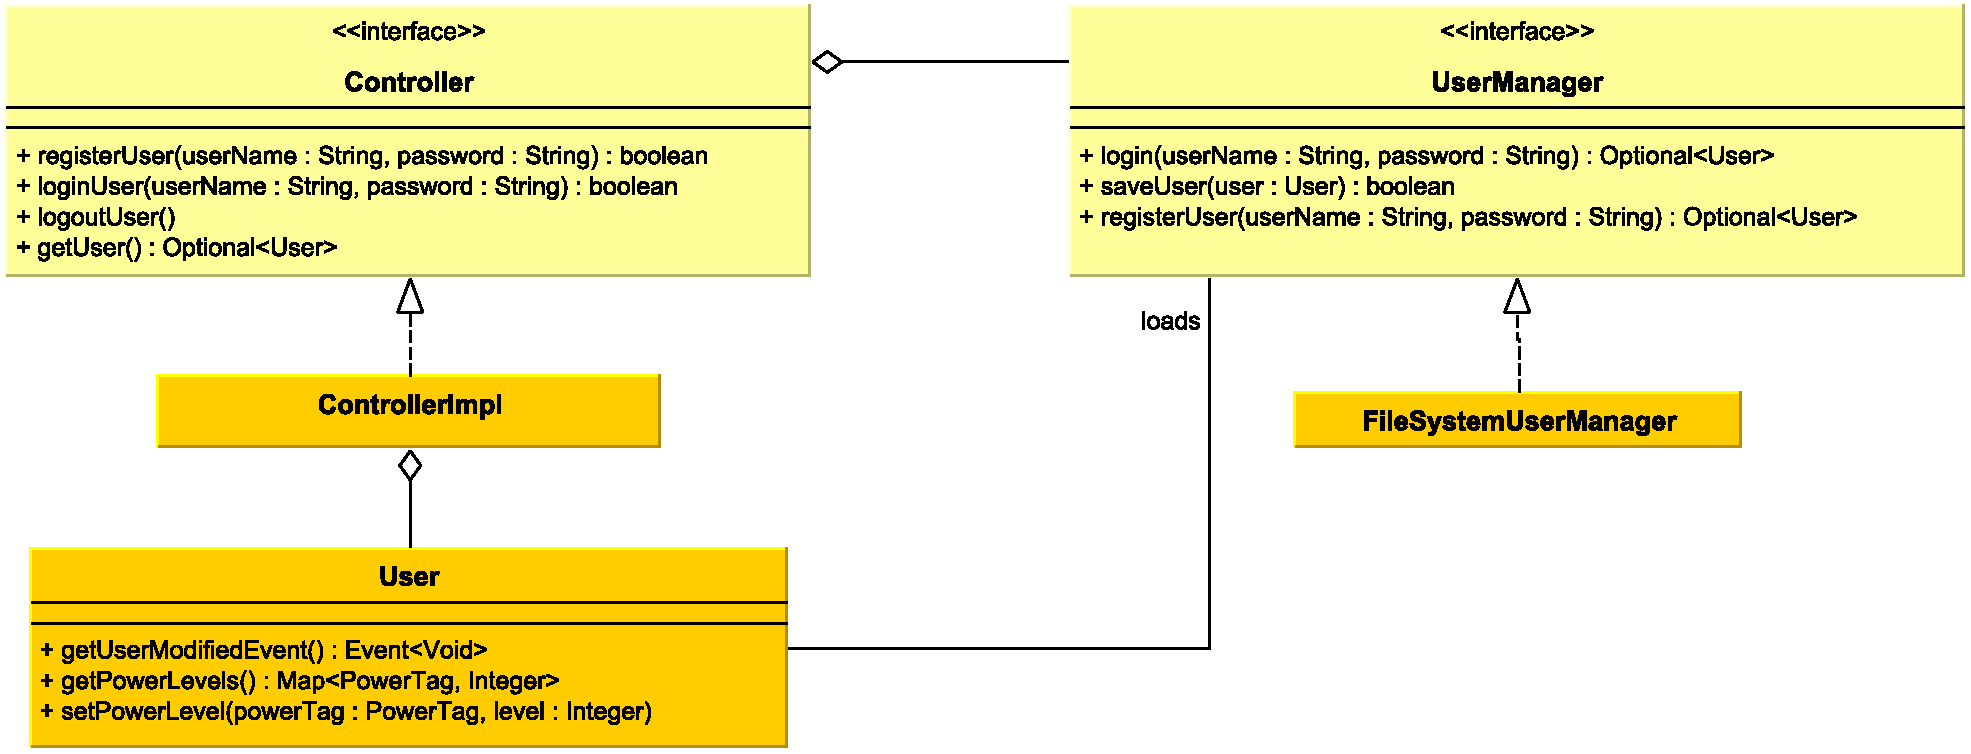
\includegraphics[width=\linewidth]{img/user}
\caption{Schema UML che mostra le relazioni tra User e UserManager}
\label{img:user}
\end{figure}

\subsubsection*{Scene Controller}
La classe astratta SceneController racchiude complessivamente i metodi per la gestione delle varie scene durante le sessioni di gioco.
L'architettura di tale classe segue il pattern di progettazione Template Method realizzato mediante due metodi della classe astratta: back() e nextScene() che richiamano al loro interno rispettivamente i due metodi astratti getPreviusScene() e getNextScene().

Questo scelta implementativa permette di lasciare alle sottoclassi la libertà di caricare scene differenti in base a quella corrente.
Tutte le scene dell'applicazione hanno modo di comunicare, richiedere informazioni ed effettuare modifiche con il Controller e la View.
All'interno della classe astratta ho deciso di creare il metodo onKeyPressed() che rappresenta l' EventHandler per la pressione di un tasto.
Questa è la parte più interattiva della classe poiché permette una differente specializzazione a seconda della scena su cui agiamo modificando il codice del tasto da premere per innescare azioni differenti.

Le classi che estendono SceneController sono numerose e riguardano separatamente ogni scena dell'applicazione.

\begin{figure}[H]
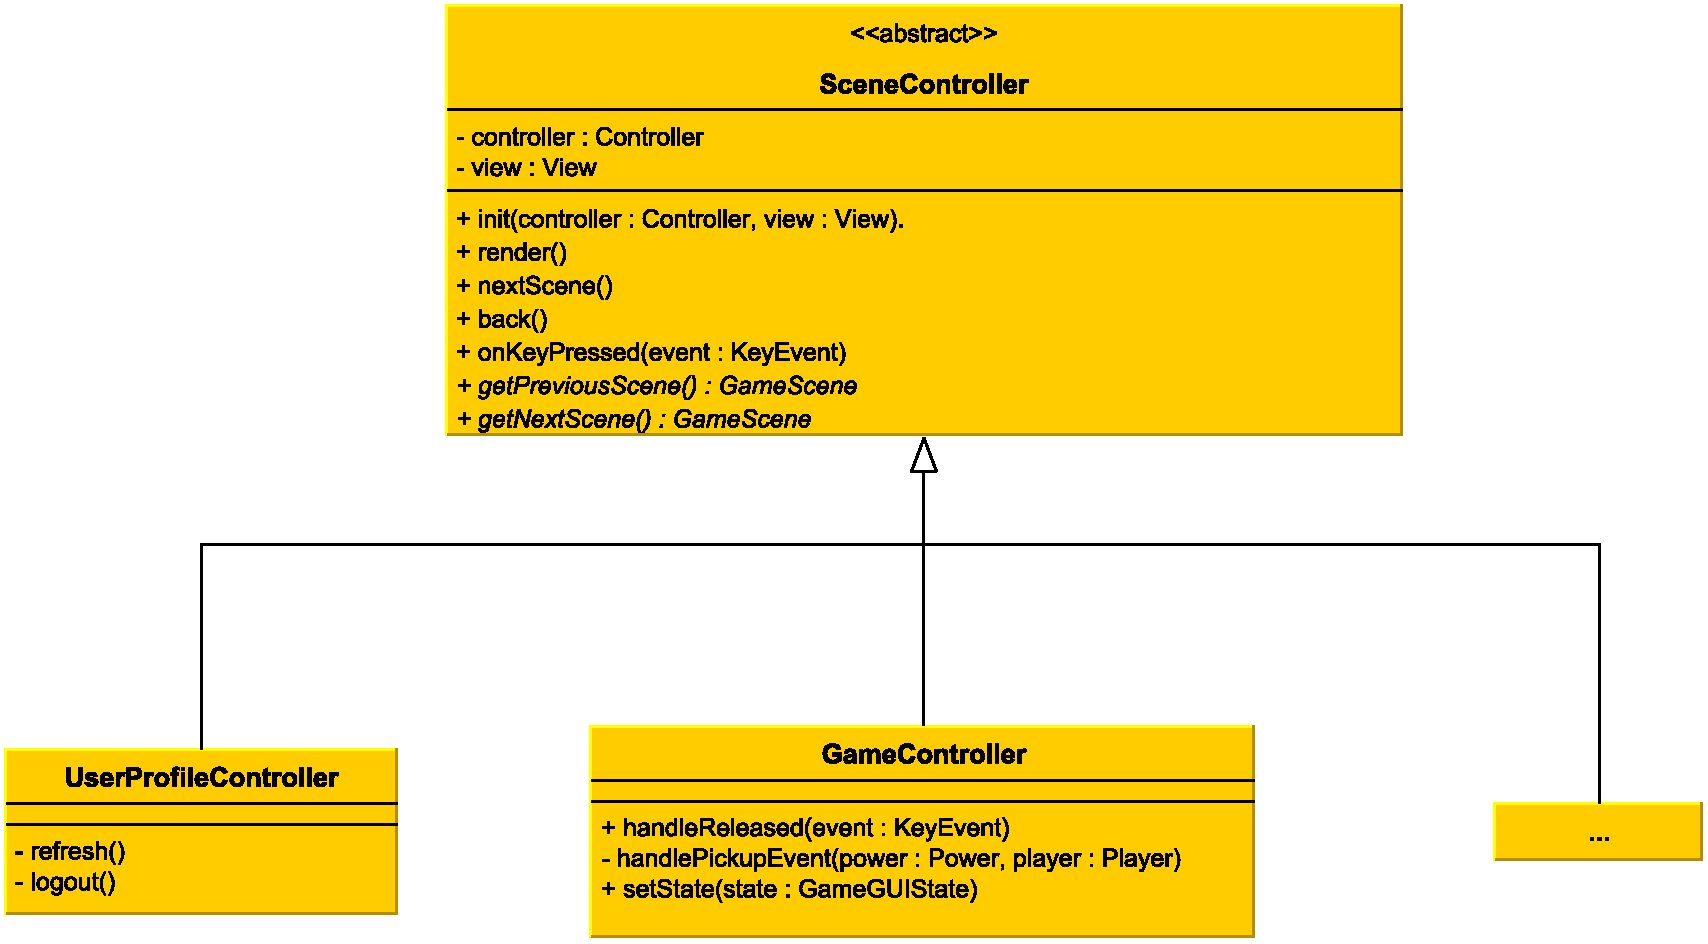
\includegraphics[width=\linewidth]{img/scene_controller}
\caption{Schema UML che mostra la gerarchia degli Scene controller}
\label{img:scenecontroller}
\end{figure}

\chapter{Sviluppo}

\section{Testing automatizzato}
Durante la fase iniziale dello sviluppo, nella quale ci siamo concentrati quasi esclusivamente sulla creazione del modello, abbiamo sentito la necessità di avere feedback sulla correttezza del lavoro svolto.
Abbiamo quindi pensato fosse un buon momento per iniziare a scrivere test automatizzati per le parti più critiche.
Per prima cosa abbiamo proceduto alla stesura di test per le collisioni (CollisionManager e Collidable), ritenuti di primaria importanza per via dell'uso della libreria dyn4j.
In seguito abbiamo optato per un test che verificasse che l'uso della Reflection per la ricerca di Component desse buoni risultati.
Successivamente ci siamo interessati alla correttezza dei meccanismi per l'input da parte dell'utente, testando in particolar modo la classe InputController.
Infine ci siamo dedicati a test per il funzionamento del Level e per l'aggiunta e rimozione di GameObject.

\section{Metodologia di lavoro}
Per sviluppare il progetto si è cercato di mantenere quanto possibile l'indipendenza delle parti assegnando aspetti distinti a ciascun membro del gruppo.
In un primo momento si è scelto di progettare nel dettaglio gli aspetti del dominio applicativo e di implementare quindi la parte Model dell'applicazione. 

Per una questione di coerenza interna la prima parte è stata svolta in collaborazione: una volta definite le interfacce principali per il Model, il Controller e la View si è passati alla definizione dei Component e lo sviluppo dei singoli GameObject nel dettaglio.
Ognuno ha quindi implementato un Component e un GameObject di cui essere responsabile.
Al fine di lavorare in parallelo ognuno ha inizialmente lavorato su un feature branch personale fino a che, una volta ottenuta una versione base funzionante dei singoli GameObject non sono stati tutti unificati su develop ed è iniziata la progettazione nel dettaglio del Controller e della View.
Degna di nota è stata l'aggiunta della GameSession che non era inizialmente prevista in fase di progettazione generale dell'applicazione, di cui però si è sentita l'esigenza per gestire in maniera più agevole tutto il flusso di gioco durante un'unica partita (fino ad esaurimento delle vite).
Parallelamente sul lato View ci si è concentrati sul rendering della scena di gioco e sulla creazione delle risorse grafiche.

Una volta ottenuta una versione "giocabile" dell'applicazione si sono iniziati a modellare i concetti di User, Leaderboard e le varie schermate di controllo in fxml, lavorando parallelamente sulla risoluzione di bug nel comportamento degli oggetti e dei poteri e sul generale del gioco.
L'ultima parte è stata principalmente dedicata alla stilizzazione grafica delle schermate e alla creazione dei livelli.

In generale la metodologia di sviluppo è stata più modulare che parallela e questo dovuto al fatto che la progettazione logica delle parti è stata abbastanza centralizzata e non affidata interamente ai singoli responsabili.
Questo, se anche in certi casi ha rallentato il gruppo, ha permesso di ottenere uno sviluppo molto coerente delle parti senza mai incontrare problemi nel processo di integrazione del codice sviluppato individualmente.

Per quanto in generale la tendenza sia stata quella di affidare la responsabilità di alcuni elementi ai singoli in alcune situazioni e specie in fase di bugfix ci sono stati piccoli interventi anche da parte di altri membri del gruppo.

In generale l'uso del DVCS è stato fatto seguendo i consigli ricevuti a lezione, cercando quindi di mantenere alcune feature isolate sui propri branch fino al loro effettivo completamento per non impattare sulla struttura principale.
Ciò è stato più facile nelle fasi iniziali di sviluppo del Model in quanto le parti erano più indipendenti, ma si è portata avanti la stessa filosofia dove possibile anche nello sviluppo complessivo dell'applicazione.

La divisione dei compiti, come già accennato nella sezione di Design di Dettaglio è la seguente:
\begin{itemize}
	\item \textbf{Burattini}: Realizzazione della meccanica di sparo, supporto per il multiplayer nel GameLoop, creazione dei Dialog per segnalare errori all'Utente, creazione delle icone dinamiche e degli elementi grafici presenti nella scena di gioco (icone dei power), rendering degli effetti dei power, gestione dell'interfaccia di potenziamento dei power, creazione e adattamento di tutte le risorse grafiche, design dei livelli della modalità storia e realizzazione in XML.
	\item \textbf{Ciarafoni}: Realizzazione dei Pickup e della struttura dei Power, gestione della leaderboard e del leaderboard manager, implementazione concreta della View.
	\item \textbf{Dente}: Creazione degli Eventi e dei Visitor, implementazione della fisica di gioco (Point2D, Vector2D, Gravity component e CollisionManager), creazione dei Wall, creazione dei decoratori per i Level, progettazione generale del rendering, implementazione del GameLoop, resize e gestione del Canvas, GameStates per gestire le varie fasi durante la partita.
	\item \textbf{Menghini}: Creazione del Player e della meccanica di Input, realizzazione del Loader per la creazione dei Livelli da file XML, implementazione della GameSession e delle sue specializzazioni, creazione del menu di pausa, decorazione delle schermate grafiche tramite CSS.
	\item \textbf{Tonetti}; Creazione della Ball e del MovementComponent, modellazione del concetto di User e UserManager, creazione dell'InstallManager, creazione delle Scene in FXML (utilizzando il tool SceneBuilder) e dei relativi Controller.
\end{itemize}

\section{Note di sviluppo}
Nello sviluppo dell'applicazione abbiamo cercato di utilizzare dove possibile gli elementi avanzati del linguaggio Java visti a lezione quali lambda expressions e Streams per avere un codice più facilmente comprensibile e semplice da scrivere.
Un caso degno di nota è quello dell'interfaccia funzionale oopang.commons.events.EventHandler, pilastro del meccanismo degli Observer presenti nel nostro progetto che è stata sempre utilizzata con l'utilizzo di lambda anche innestate.

Dove utile, in particolare per gli User e la Leaderboard, si è fatto uso di Optional e anche in tal caso si è preferito la creazione di lambda per programmare le azioni da eseguire sugli optional stessi.
In generale inoltre si è fatto uso di alcune delle interfacce funzionali fornite dal linguaggio Java quali Consumer e Supplier, molto utili per poter delegare delle operazioni senza creare veri e propri oggetti dedicati.

\subsection*{Samuele Burattini}
Nel mio lavoro personale, oltre agli elementi sopracitati, ho utilizzato alcune funzionalità di JavaFX per la realizzazione dei blocchi dinamici per l'interfaccia utente all'interno della JavaFXUIFactory e per la realizzazione dei Dialog. Per quest'ultimi ho utilizzato degli snippet di codice presi da un tutorial reperito in rete a questo \href{http://code.makery.ch/blog/javafx-dialogs-official/} {link} .

Ulteriori competenze esterne a quelle specifiche del corso di programmazione ad Oggetti includono l'elaborazione delle risorse grafiche principalmente tramite Photoshop e la produzione dei file XML per la codifica dei livelli.

\subsection*{Nicholas Ciarafoni}
All'interno della gestione delle Leaderboard ho implementato l'interfaccia Serializable, trasformando così l'intera classe in una stringa di byte, questo flusso creato dunque viene poi caricato e salvato su file binario in modo da garantire la persistenza.

Ho inserito un Optional$\langle$Integer$\rangle$ per controllare se nella Leaderboard l'ultimo record registrato è stato aggiunto alla "top ten", se è presente tengo traccia dell'indice del record.

Nei Power ho fatto uso del pattern di programmazione Visitor, con il metodo visit() ho verificato per esempio nel Power Dynamite, se all'interno del livello erano presenti degli oggetti di tipo Ball e poi ne invocavo la distruzione, analogamente con il Power Freeze, verificavo se all'interno del level avevo oggetti di tipo Ball e di tipo Player.
Avendo riscontrato dei problemi nell'accumulo di power differenti ho avuto la necessità di impostare e tenere aggiornato un counter di "invulnerabilità" che il Player ha attive su di se, tramite questo valore scelgo se disattivare il la collisione del Player con le Ball.

\subsection*{Francesco Dente}
Nella fase di sviluppo ho avuto a che fare, per la gestione delle collisioni, con una libreria esterna per la simulazione della fisica.
A seguito di una fase di documentazione sono quindi riuscito a informarmi sulle sole parti necessarie per la rilevazione delle collisioni e a integrarle col nostro sistema.

Ho avuto a che fare anche con meccanismi propri di JavaFX come il binding, usato per garantire un resize fluido della finestra.

In più ho implementato un meccanismo di caching delle immagini sfruttando il pattern \textbf{Proxy}.

\subsection*{Lorenzo Menghini}

\subsubsection*{GameSession}
La GameSession è parte del cuore dell'applicazione ed ha un ruolo di contenimento e passaggio di informazioni.
Modella il concetto di sessione di gioco e contiene istanze della View, del Model, e del GameLoop; essendo interfacciata con il controller funge da ponte di comunicazione tra quest'ultimo e gli altri pilastri dell'architettura del software. Questo ci permette in modo pulito di gestire delle fasi cruciali del gioco come l'evento di morte o la gestione dell'inizio di una nuova partita, dando indicazioni anche alla View sul comportamento da tenere (quali scene caricare, ad esempio).
Facendo uso del pattern Observer, nella GameSession vengono innescati o "triggerati" degli eventi quali la creazione di un livello o la fine di una partita che generano azioni rilevanti sul Model o in generale su tutte le entità reistrate a questi due Eventi.

Come spiegato nell'architettura di dettaglio è stato necessario suddividere l'implementazione in due classi differenti, a seconda della modalità di gioco da avviare (Survival o Story) mantenendo comunque le azioni comuni implementate nella classe astratta, poichè le notevoli differenze come ad esempio modalità di morte (nella Survival non esiste il "timeout") o caricamento del livello (gestito poi in parte dall'XMLLevelLoader) portavano ad una relizzazione più pulita e funzionale tramite questa suddivisione.
La startNewLevel è un metodo chiave poichè incorpora quella che è la creazione di una nuova scena di gioco: crea le Map per contenere informazioni sui player (uno o due a seconda della scelta dell'utente) e i relativi InputWriter, si occupa di aggiungere la figura del Player al livello (compito scorporato del LevelLoader poichè la figura del Player non è variabile a seconda del livello) e riceve dal LevelLoader il livello caricato, registra quest'ultimo all'evento di terminazione della partita e indica alla view, passandogliene l'istanza, che il livello è stato creato; ma cosa più importate crea e accende il GameLoop che è il motore di tutto il gioco.
Per quanto riguarda la fase di terminazione di una partita, la GameSession si occupa di fermare il flusso di gioco e ricevere i dati relativi ai risultati ottenuti (score e anche modalità di morte o vittoria).

A questo punto darà l'input alla view di caricare la scena adatta a seconda del tipo di terminazione ottenuta.
Come costrutti avanzati del linguaggio ho fatto uso di Optional, della reflection per la costruzione della EnumMap e anche di lambda che rendono il codice più leggibile ed ordinato.

\subsubsection*{XML Level Loader}
L'XMLevelLoader ha il compito di "parsare" le informazioni necessarie alla costruzione della scena di gioco da un file esistente.
Per la strutturazione dei livelli ho deciso di usare il meta linguaggio XML che mi permette tramite i tag di poter leggere il file con più libertà di azione.
Questo mi ha portato a scrivere della funzioni di utility modulari per catturare nel file le parti che mi interessavavo specificandone nella chiamata i tag da cercare e la sorgente di partenza.
Facendo uso del LevelBuilder (che implementa il patter Builder) ho construito il livello pezzo per pezzo ad ogni lettura di informzioni per poi passarlo dopo aver fatto la build al LevelData che contiene inoltre informazioni sullo sfondo e sulla texture dei muri di gioco.
Per implmentare in modo efficace la lettura ho fatto uso della libreria esterna DOM che mette a disposizione metodi, interfacce e classi molto utili per la modellazione dei dati.

I due metodi pubblici (loadStoryLevel e loadInfiniteLevel) chiamano all'interno un metodo privato che, facendo uso di un Optional e a seconda della sua presenza o meno tra i parametri al momento della chiamata, legge in modo differente il file poichè conosco a priori la presenza o meno di tag all'interno del file dell'infiniteLevel.
Per la gestione dei PowerUps agisco in modo leggermente diverso (non per quanto riguarda la lettura ma per l'utilizzo del builder) chiamando, attraverso l'uso di lambda, dei metodi di creazione sulla powerFactory.

\subsubsection*{Input}
Per spiegare il funzionamento della gestione dell'input da parte dell'utente occorre procedere per gradi: alla cattura dell'evento di pressione un tasto specifico da parte della view viene invocato il metodo sendcommand nel controller che, attraverso l'uso di una lambda, invia al GameLoop (passando per la GameSession che in questo caso funge da ponte) il comando da inserire nella BlockingQueue per poi farlo processare dal metodo processInput al successivo update.
Durante l'esecuzione della processInput il comando inserito nella Queue viene prelevato e passato all'InpuWriter che si occuperà di scrivere i valori corrispondenti relativi al comando.

A questo punto sarà responsabilità dell'InputReader leggere i valori scritti e renderli disponibili all'InputComponent avendone quest'ultimo un'istanza.
Alla chiamata dell'update sull'InputComponent viene invocato un metodo privato handleInput che, attraverso l'uso di Consumer parametrizzati, gestisce il settaggio di cambi di direzione o richiesta di sparo generando quindi nei GameObject interessati un cambio effettivo dei parametri.


\subsection*{Francesca Tonetti}
Nello sviluppo delle parti di applicazione del gioco di cui mi sono occupata, oltre ad aver incluso gli elementi di programmazione comuni a tutti i componenti del gruppo, mi sono impegnata nella gestione di serializzazione dello User, la gestione dei dati sul filesystem e parte delle realizzazione delle viste grafiche.
In riferimento a quest'ultimo ho utilizzato il programma SceneBuilder per la creazione di tutte le scene di gioco, alle quali ho associato riferimenti al controller mediante l'FXMLLoader collocato nella classe SceneLoader.

Per quanto riguarda la gestione degli utenti, la classe User di riferimento implementa Serializable che definisce il meccanismo di salvataggio dei dati su file relativi all'utente mediante uno stream binario in modo che ad ogni sessione vengano ripristinati, per questo sono state approfondite le classi java.io.FileInputStream e java.io.FileOutputStream.
Per la creazione di una cartella di installazione ho implementato un InstallManager usando le API di Java.

Infine un'altro aspetto di sviluppo interessante è il meccanismo di hashing applicato alle password dell'utente, per proteggere in maniera minimale i dati sensibili dell'utente stesso.




\chapter{Commenti finali}

\section{Autovalutazione e lavori futuri}


\subsection*{Samuele Burattini}
Ho trovato il lavoro sul progetto molto istruttivo e utile in quanto dà la possibilità di cimentarsi per la prima volta con la ideazione e realizzazione di un software complesso. La fase che ho ritenuto più stimolante è stata quella della progettazione dell'applicazione, in particolare le fasi di analisi del dominio e strutturazione del Model. Questa parte mi ha visto anche particolarmente attivo in quanto, un po' per una questione di tempistiche in relazione alla sessione invernale, un po' per una maggiore dimestichezza con i costrutti tipici della programmazione a oggetti la progettazione ha impegnato principalmente me e Francesco.
Particolarmente interessante è stata la costruzione di una struttura che fosse il più possibile modulare e che rendesse semplice fare modifiche e aggiunte senza impattare pesantemente sul resto. Indubbiamente non tutto è stato svolto nel migliore dei modi anche soprattutto per una questione di inesperienza ed in particolare per le sezioni del Controller e della View più lontani dalla programmazione "classica".

Per quello che riguarda lo sviluppo ho lavorato bene con il gruppo, e ho apprezzato l'utilizzo del DVCS che introduce ad una metodologia di lavoro molto più vicina al mondo professionale, nonostante un primo periodo di incertezza per familiarizzare con i comandi con il tempo si è rivelato uno strumento indispensabile.
Nonostante fossimo un gruppo numeroso non abbiamo avuto grandi difficoltà nel suddividere il lavoro e siamo riusciti a tenere quasi sempre il passo in maniera uniforme, unica pecca è stata la scarsa indipendenza dei singoli che ci ha "costretto" a vederci periodicamente per fare il punto della situazione e andare avanti nello sviluppo. Questo probabilmente è dipeso in parte anche a causa del fatto che avendo progettato all'inizio la struttura generale è stato più difficile per gli altri inserirsi nella stessa ottica, ma anche semplicemente da un livello disomogeneo di praticità nell'utilizzo del linguaggio.

Mi ritengo molto soddisfatto del lavoro svolto sia personalmente che dal gruppo, credo di aver lavorato bene e di essere riuscito a mettere in pratica quanto appreso in quest'anno affinando ulteriormente gli strumenti fornitici durante il corso. Quando all'inizio del semestre ci erano stati presentati gli elaborati degli anni passati ero rimasto particolarmente colpito e non pensavo sarei riuscito a raggiungere risultati dello stesso livello.

Reputo l'esperienza generale estremamente formativa e considero l'elaborato finale un prodotto completo, mi piacerebbe continuare nello sviluppo (anche se non so se sarà possibile considerando gli altri impegni di questo semestre) inserendo altri elementi per rendere più vario il gameplay come l'aggiunta di altri GameObjects quali scale, muri distruggibili e palle o pistole con comportamenti differenti sfruttando l'architettura dei Component già predisposta. 

\subsection*{Nicholas Ciarafoni}
L'idea di portare come prova pratica un progetto di grosse dimensioni è interessante, peccato che manchino le giuste guide per portare a termine un gioco di questa tipologia, in molte parti sarebbe stato utile avere affianco un tutore che ci instradasse meglio al concetto di gioco, e delle sue caratteristiche principali, in particolare per quel che riguarda la View.
A lezione ci siamo concentrati molto sulla teoria, e nel laboratorio a metterla in pratica, sarebbe carino, provare a creare dei giochi in laboratorio, dove allo stesso tempo si mette in pratica la teoria seguita a lezione piuttosto che completare esempi preimpostati.

Nel processo di sviluppo ho avuto dei problemi nel capire la struttura generica del progetto all'inizio, cosa che ho fatto subito capire al gruppo di lavoro, e in alcune parti ho avuto la necessità di avere affianco una persona che sapesse guidarmi nelle parti di codice scritto, tempestandola di domande ad ogni passo.
Troppa insicurezza in me e confusione mi hanno portato a volte in situazioni di stallo dove non sapevo proprio come continuare il mio lavoro, poi nel momento in cui qualcun altro del gruppo mi affiancava riuscivo a portare a termine i punti che progressivamente ci impostavamo.

L'insicurezza mi ha portato anche a non riuscire in una delle mie challenge personali, quello di inserire la musica, e il poco tempo rimasto non ha giocato a mio favore.
Per uno sviluppo futuro pensavo di inserire appunto degli effetti sonori, musica di gioco, e vari potenziamenti aggiuntivi come per esempio la possibilità di avere potenziamenti fluttuanti e collezionabili a contatto con l'HookShot o potenziamenti nascosti dentro muri distruttibili.

\subsection*{Francesco Dente}
Questo progetto ha messo a dura prova le capacità di noi studenti e ci ha messo a confronto con difficoltà particolari tipiche del mondo del lavoro.
Grazie al lavoro svolto sono riuscito a comprendere più a fondo le parti veramente critiche della gestione di un software complesso e ho ottenuto una maggiore dimestichezza coi mezzi messi a disposizione dal mondo informatico.
Particolarmente istruttivo per me è stato l'utilizzo del DVCS che, come per tutti i nuovi all'argomento, era difficilmente apprezzabile inizialmente, ma che si è poi ovviamente rivelato indispensabile.

Ritengo che le mie esperienze passate nello sviluppo di videogiochi per puro hobby abbiano influenzato pesantemente le mie scelte progettuali, nonostante le nuove conoscenze apprese a lezione abbiano sicuramente aggiunto un occhio critico sulle limitazioni dei miei vecchi mezzi.
In passato infatti non ero mai estremamente orientato alla modularità e alla flessibilità del codice, ed inoltre tendevo sempre a buttarmi rapidamente sulla scrittura piuttosto che organizzare e progettare in primo luogo.
Ritengo dunque che questo progetto abbia corretto (almeno in parte) questo mio "difetto".

Penso che il lavoro sia stato svolto in maniera positiva nonostante la disomogeneità delle conoscenze che spesso ci vedeva rallentare per permettere di mantenere il passo comune.

Credo infine che questo progetto possa essere un buon trampolino per lavori futuri, spero anche con l'appoggio di colleghi universitari, e che ci serva sia come conferma di ciò che sappiamo fare che come "lezione" per non ripetere errori già commessi.

\subsection*{Lorenzo Menghini}
Ho trovato la realizzazione del progetto uno degli aspetti più stimolanti affrontati fin'ora nel mio percorso universitario: mi ha permesso di realizzare ancora meglio cosa significa lavorare in un team di sviluppo e i relativi vantaggi/svantaggi di non essere da solo davanti al computer.
A causa del prolungarsi della sessione invernale non ho potuto affrontare in modo dettagliato come avrei voluto la fase di progettazione che è stata presa in carico più in dettaglio da Samuele e Francesco. Nonostante un primo periodo di ambientazione per poter capire a pieno le sfaccettature architetturali sviluppate dai miei compagni, credo di essermi inserito bene nel lavoro e di aver portato un bel contributo alla realizzazione dell'elaborato.

Sono stato in grado di lavorare in modo individuale senza problemi e in alcuni casi ho supportato i miei compagni nella comprensione del codice del progetto nel caso avessero difficoltà.
Grazie ad alcune conoscenze pregresse, esterne al corso di Programmazione ad Oggetti, ho scritto dei file CSS per la stilizzazione delle varie schermate di gioco prendendomi carico di buona parte di questa sezione di progetto.

In conclusione ho trovato questo percorso particolarmente formativo sia dal punto di vista tecnico/implementativo (in particolare per l'importanza dell'utilizzo corretto dei pattern), sia dal punto di vista organizzativo per la gestione del carico di lavoro in gruppo.
Mi ha aiutato ad apprendere in modo efficace e funzionale l'utilizzo di un DVCS comprendendo la sua indispensabile presenza all'interno di un progetto codiviso tra più sviluppatori.
Ringrazio i miei compagni per aver condiviso questo bellissimo progetto insieme e siamo sicuramente tutti soddisfatti di quello che questa cooperazione ha portato alla luce, a parer mio un bellissimo gioco, stimolante e quasi "addictive". 

Ho intenzione di continuare nello sviluppo dell'applicativo aggiungendo una leaderboard globale informandomi prima sull'implementazione in PHP dei file necessari a creare un collegamento in rete accessibile a tutti gli utenti per rendere la user experience ancora più competitiva.

\subsection*{Francesca Tonetti}
Questo progetto è stato frutto di molto lavoro coeso fra tutti i componenti del gruppo.
Se pur spesso sia stato faticoso completare autonomamente parti di sviluppo del gioco, grazie all'aiuto dei compagni e ad incontri pomeridiani, mi ritengo ripagata dal risultato finale ottenuto e posso dirmi estremamente soddisfatta.

Inizialmente la proposta di realizzare un gioco non mi ha entusiasmato non solo perché non sono mai stata appassionata al mondo dei videogiochi, ma soprattutto perché avevo molti dubbi riguardo le mie abilità di programmazione in quanto le conoscenze in linguaggio Java non le ritenevo abbastanza consistenti da poter completare un elaborato di questo genere.
Arrivata però al completamento del progetto, penso sia stato estremamente utile cimentarsi in un gioco così corposo e strutturato di fatti questo mi ha permesso di ampliare le mi conoscenze anche per quanto riguarda altri aspetti implementativi come le parti grafiche che compongono le scene di OOPANG.
Infatti una tra le cose che mi ha più interessato è stata proprio quella di poter lavorare sugli aspetti più grafici cimentandomi con un programma che non conoscevo, SceneBuilder, e sfruttando la mia vena più artistica dando opinioni come ad esempio sulle scene, i colori, la scelta delle icone per i powers o il player.

Complessivamente penso sia stato molto piacevole lavorare in gruppo sia perché ci ha sempre permesso di confrontarci vicendevolmente ma soprattuto per poter chiedere aiuto ogni qualvolta non fossimo sicuri di svolgere in maniera corretta il lavoro assegnato, anche perché per quanto riguarda la suddivisione dei compiti non è mai stata cosi netta e precisa la linea tra il lavoro di un compagno e l'altro.
La costanza e le abilità di alcuni componenti del gruppo penso siano state essenziali e di grande aiuto per veder progredire in maniera costante il progetto, senza mai perdere di vista gli obbiettivi prefissati effettuando un check periodico del lavoro.
Questo mi ha permesso ancor più di capire quanto per me sia punto di forza sapere di avere attorno un team di persone con le quali potermi confrontare attivamente, ed è un aspetto che anche in futuro spero di ritrovare nel mondo del lavoro.

Infine penso che il mio lavoro sia stato utile per la realizzazione del gioco, ho sempre cercato di svolgere i compiti assegnati in maniera precisa e puntuale senza dimenticare il fatto che non solo fossi responsabile di ciò dovevo compiere, ma che far del proprio meglio avrebbe aiutato me ed i miei compagni.
Spero un domani, con la collaborazione dell'intero gruppo, si possano migliorare altri aspetti del gioco magari aggiungendo altri livelli associati alla creazione di power nuovi, per rendere l'applicazione più innovativa.

\section{Difficoltà incontrate e commenti per i docenti}
La principale difficoltà che abbiamo riscontrato nello sviluppo del progetto è stata la progettazione di una parte View composta da più schermate collegate tra loro. Crediamo che sia una sezione importante e che meriti un approfondimento nella trattazione del corso in quanto raramente ci si troverà a creare sistemi a singola finestra. 
In più riteniamo che sarebbe stato meglio approfondire di più l'uso di DVCS Git e del repository online Bitbucket per potersi esercitare, introducendoli anche prima di quanto è stato fatto in modo che gli studenti possano acquisire più dimestichezza ed utilizzare da subito questi strumenti in maniera efficace visto che si sono rivelati incredibilmente utili.


\chapter{Apppendice A}
\section{Guida Utente}

\subsection*{Scopo del gioco}
Il giocatore ha come obiettivo quello di distruggere le palle generate dal gioco, attraverso un arpione,  cercando di non essere mai colpito. 
Ad ogni sparo il proiettile può permettere di distruggere le palle che vengono toccate anche con la corda, una volta colpite queste ultime si sdoppiano dimezzandosi fino a quando non raggiungono un raggio minimo e spariscono.

\subsection*{Modalità di gioco}
Esistono due modalità di gioco
\begin{itemize}
	\item \textbf{Tour Mode}: il giocatore ha lo scopo di completare tutti i 17 livelli nel tempo prestabilito per ogni livello.
	\item \textbf{Survival Mode}: il giocatore ha lo scopo di sopravvivere il maggior tempo possibile man mano che il numero di palle aumenta.
\end{itemize}
In entrambe le modalità lo scopo è quello di accumulare più punti possibili per guadagnare esperienza.
Colpire le palle in serie senza mai sbagliare, permette di aumentare il punteggio ricevuto ad ogni colpo.

\subsection*{Poteri attivabili}
\begin{itemize}
	\begin{figure}[H]
			\item
			
\includegraphics[width=0.05\linewidth]{img/1}
			\label{img:doubleshot}
			\textbf{DOUBLESHOT}

			Permette al player di sparare due volte di fila. 

  			\underline{POTENZIAMENTO}: Permette al player di sparare tre volte di fila.
	\end{figure}
	\begin{figure}[H]
			\item
			
\includegraphics[width=0.05\linewidth]{img/2}
			\label{img:sticky}
			\textbf{STICKYSHOT}

			Il proiettile si attacca al muro per tre secondi.

 			\underline{POTENZIAMENTO}: Permette al player di sparare due volte di fila.
	\end{figure}
	\begin{figure}[H]
			\item
			
\includegraphics[width=0.05\linewidth]{img/3}
			\label{img:freeze}
			\textbf{FREEZE}

			Tutte le palle si fermano per un tot di tempo e il player è invulnerabile.

 			\underline{POTENZIAMENTO}: Aumenta la durata di 0.5 secondi ad ogni livello (MAX 5).
	\end{figure}
	\begin{figure}[H]
			\item
			
\includegraphics[width=0.05\linewidth]{img/4}
			\label{img:doublespeed}
			\textbf{DOUBLESPEED}
			
			Tutte le palle vengono rallentate come se il player andasse super veloce.

 			\underline{POTENZIAMENTO}: Aumenta la durata di 0.5 secondi ad ogni livello (MAX 5).
	\end{figure}
	\begin{figure}[H]
			\item
			
\includegraphics[width=0.05\linewidth]{img/5}
			\label{img:shield}
			\textbf{TIMEDSHIELD}

			Crea una bolla intorno al player che lo rende invulnerabile.

 			\underline{POTENZIAMENTO}: Aumenta la durata di 0.5 secondi ad ogni livello (MAX 5).
	\end{figure}
	\begin{figure}[H]
			\item
			
\includegraphics[width=0.05\linewidth]{img/6}
			\label{img:dynamite}
			\textbf{DYNAMITE}

			Fa esplodere tutte le palle in gioco una volta.

 			\underline{POTENZIAMENTO}: La dinamite colpisce tante volte quanto il livello associato (MAX 3).
	\end{figure}
\end{itemize}

\subsection*{Controlli}

\subsection*{Schermata di gioco principale}
\begin{figure}[H]
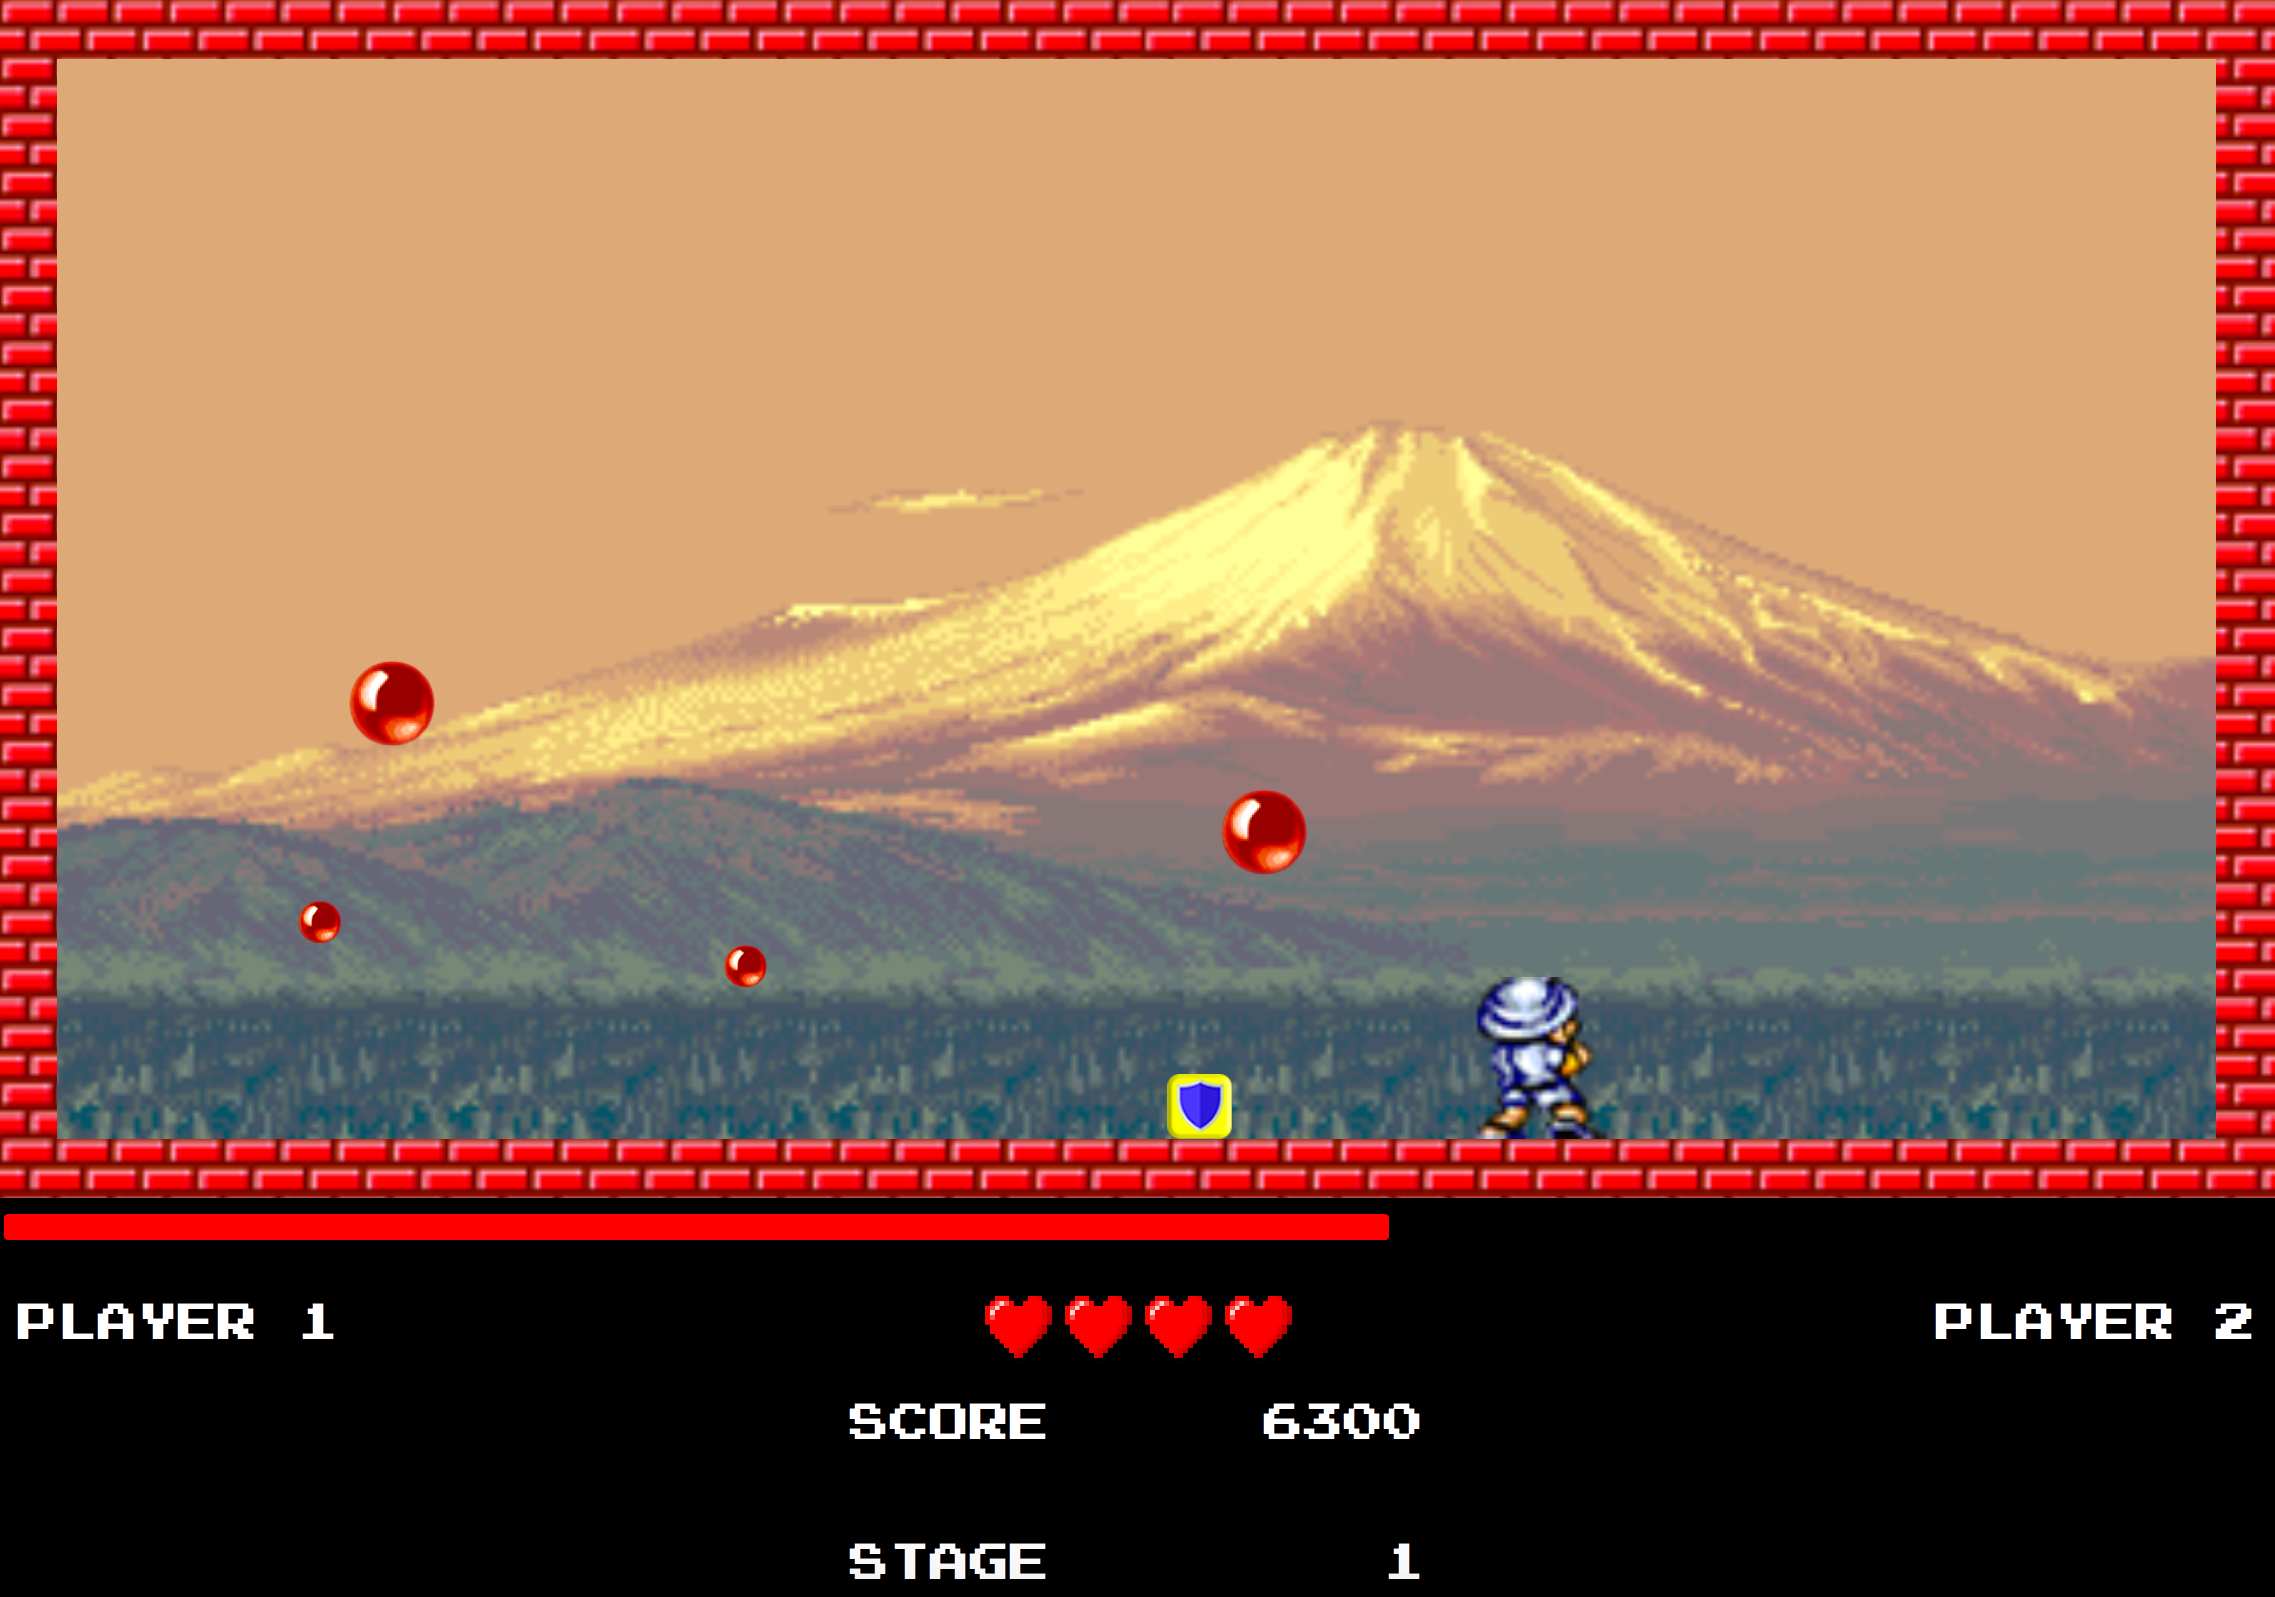
\includegraphics[width=\linewidth]{img/7}
\label{img:decorator}
\end{figure}

\begin{itemize}
\item \textbf{CUORI}:     vite del player
\item \textbf{SCORE}:     punteggio calcolato in base al numero di palle distrutte ed agli
             oggetti raccolti
\item \textbf{STAGE}:     livello raggiunto dall'utente
\item \textbf{PLAYER1/2}: nome del player sotto al quale un box contiene i pickup a tempo attivi durante la   
             sessione di gioco, mentre accanto al nome appare l'icona della pistola in uso.
\end{itemize}

\subsection*{Profilo Utente}
\begin{figure}[H]
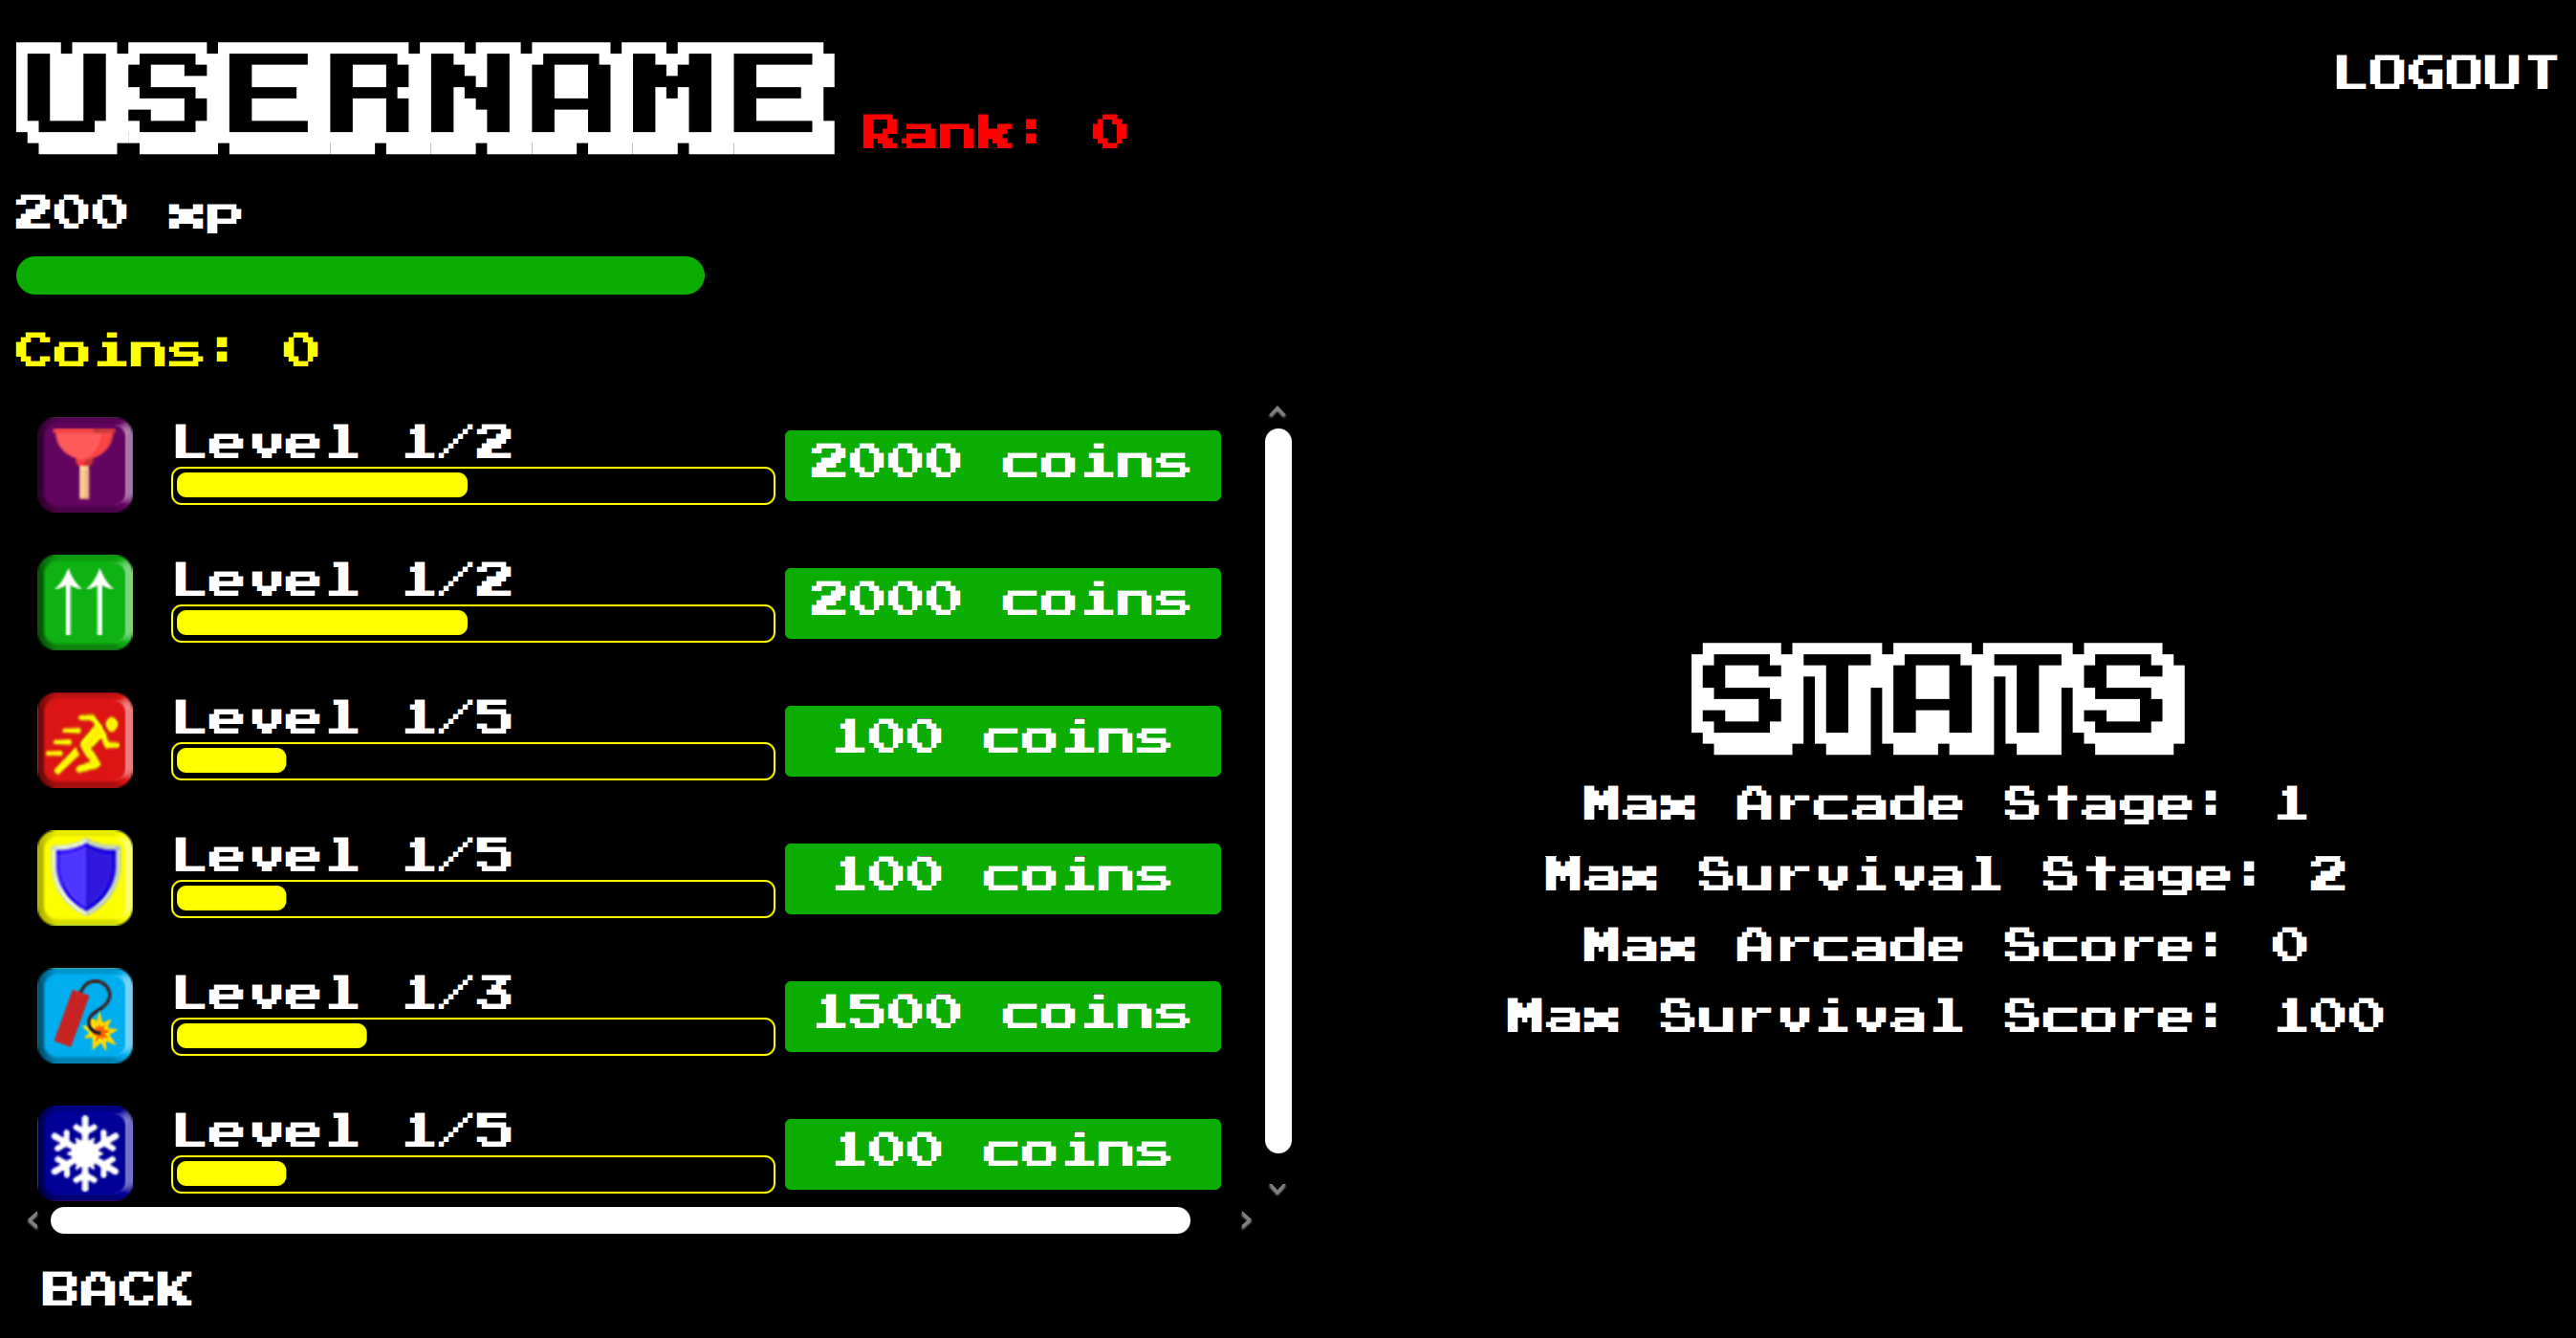
\includegraphics[width=\linewidth]{img/8}
\label{img:decorator}
\end{figure}

\begin{itemize}
\item \textbf{USERNAME}:     nome utente
\item \textbf{RANK}:     rank dell'utente calcolato in base ai punti esperienza guadagnati
\item \textbf{XP POINTS}:     punti esperienza guadagnati per raggiungere il rank successivo
\item \textbf{COINS}: 	monete accumulate tramite le ricompense per acquistare i potenziamenti dei power
\item \textbf{POWER BOX}: 	Schermata di potenziamento per i power con il rispettivo indice di livello e costo di potenziamento
\end{itemize}


\end{document}

